\chapter{Experimental Setup}
\label{ch:test_setup}
As there is no experimental data of different overflow shapes, the main priority is to test various overflow shapes. Thanks to previous research done at the Technological University of Delft, a 25$m^3$ rectangular reservoir was available to do experimental tests. A physical description is given in section \ref{sec:phy}. Next to that, several parameters are explained in section \ref{sec:para} and all experimental scenario's are shown in section \ref{sec:scenario}. To do the experiments efficient and in a controllable way, a chronological work plan is made which can be found in Appendix \ref{app:work_plan}. The main focus of the experiments are:

\begin{itemize}
    \item Try three different overflow shapes (round \& two different rectangle aspect ratios) and see by concentration measurements if the concentration distribution in 2D is different.
    \item By video imaging, the angle of the plume can be obtained which can be translated to an entrainment factor which explains the amount of entrainment between the plume and surrounding water.
\end{itemize}

\newpage
\section{Physical description experimental setup}
\label{sec:phy}
In this section, all parts that make the experimental setup are described. A schematic overview of the used test setup is shown in Appendix \ref{app:experimental_setup}.  \newline \newline
\noindent\textbf{Reservoir}\newline
\noindent A 25$m^3$ rectangular reservoir is used to perform the experimental tests in which is shown in figure \ref{fig:reservoir_tank}. During the tests, the reservoir is filled with tap water. At the top, a frame is positioned to slide the overflow in the right place. The tests can be visually assessed by the glass windows on the reservoir.


\begin{figure}[ht!]
    \centering
    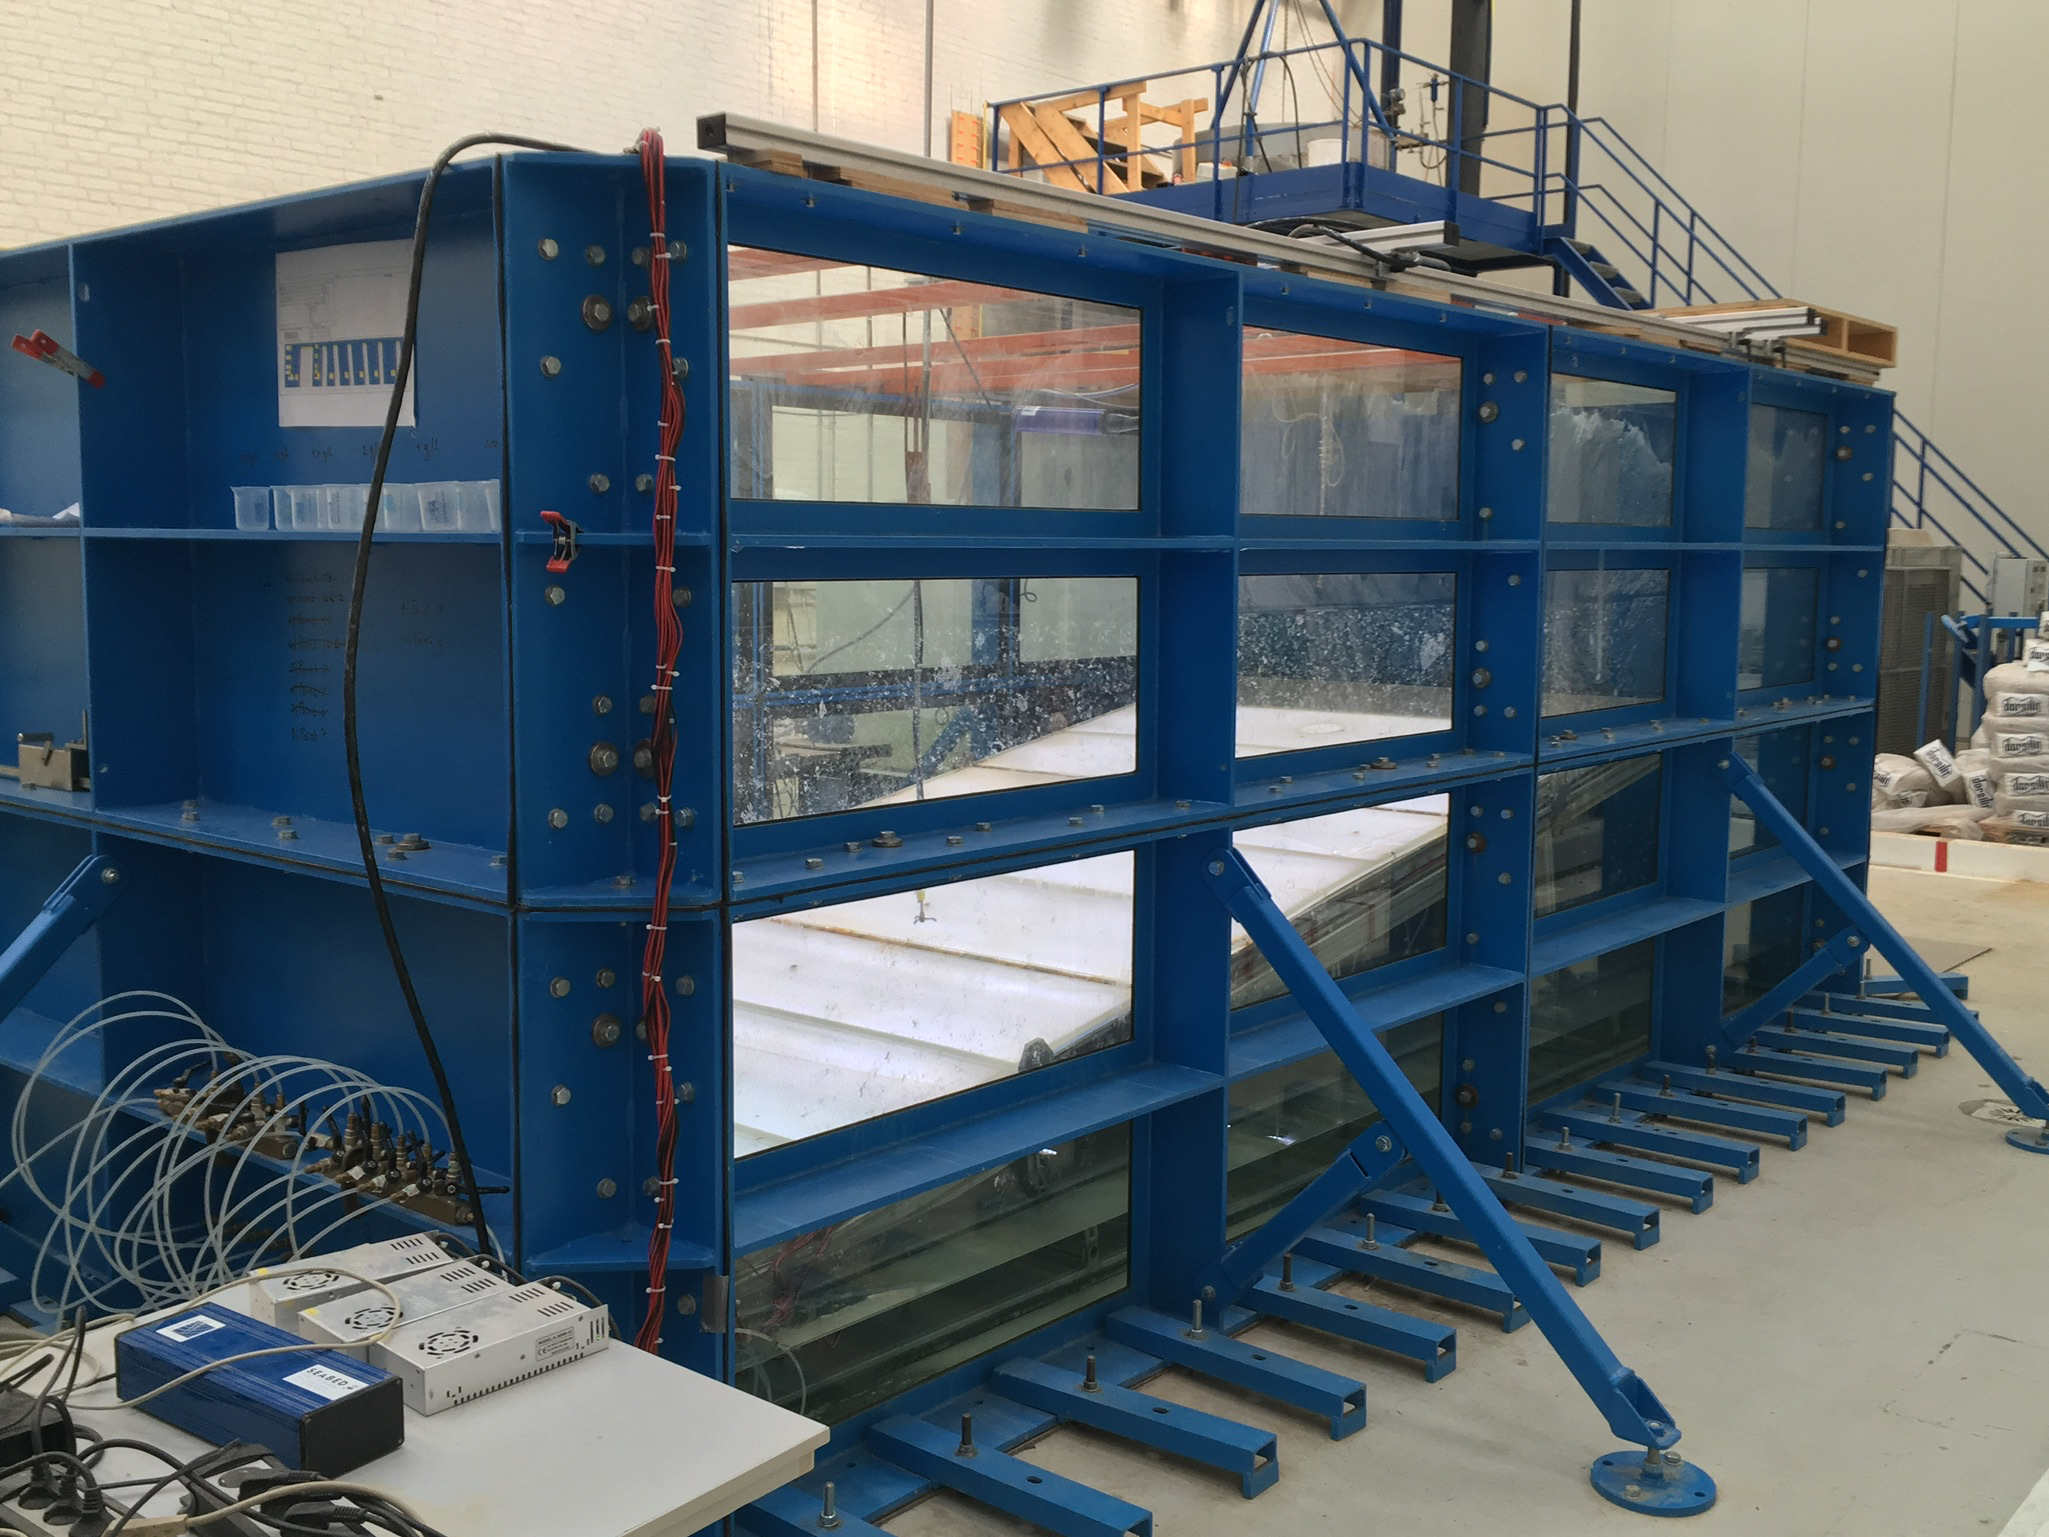
\includegraphics[width=\textwidth]{Images/Reservoir_tank.jpg}
    \caption{25$m^3$ rectangular reservoir at TU Delft}
    \label{fig:reservoir_tank}
\end{figure}


\noindent\textbf{Mixing tank} \newline
%Manier van mixen
%Pompen (in tank en 'vervoer')
\noindent The mixing tank (1.5m x 0.78m x 1m) is a perspex tank which is divided in two equal sections which both have a volume of approximately 500L. In one section, water and sediment are mixed to reach a certain mixture density which is done by hand in combination with a submersible pump. This mixture is pumped from the mixing tank with a small stainless steel flexible impeller pump, with a maximum flow of 20L/min, to the reservoir through a 10mm (inside)diameter pipe. During an experimental test, the other section of the mixing tank can be prepared for the next run and so create another mixture, this to decrease preparation time during testing. An overview is shown in figure \ref{subfig:mixing_tank}.


\begin{figure}[ht!]
  \centering
  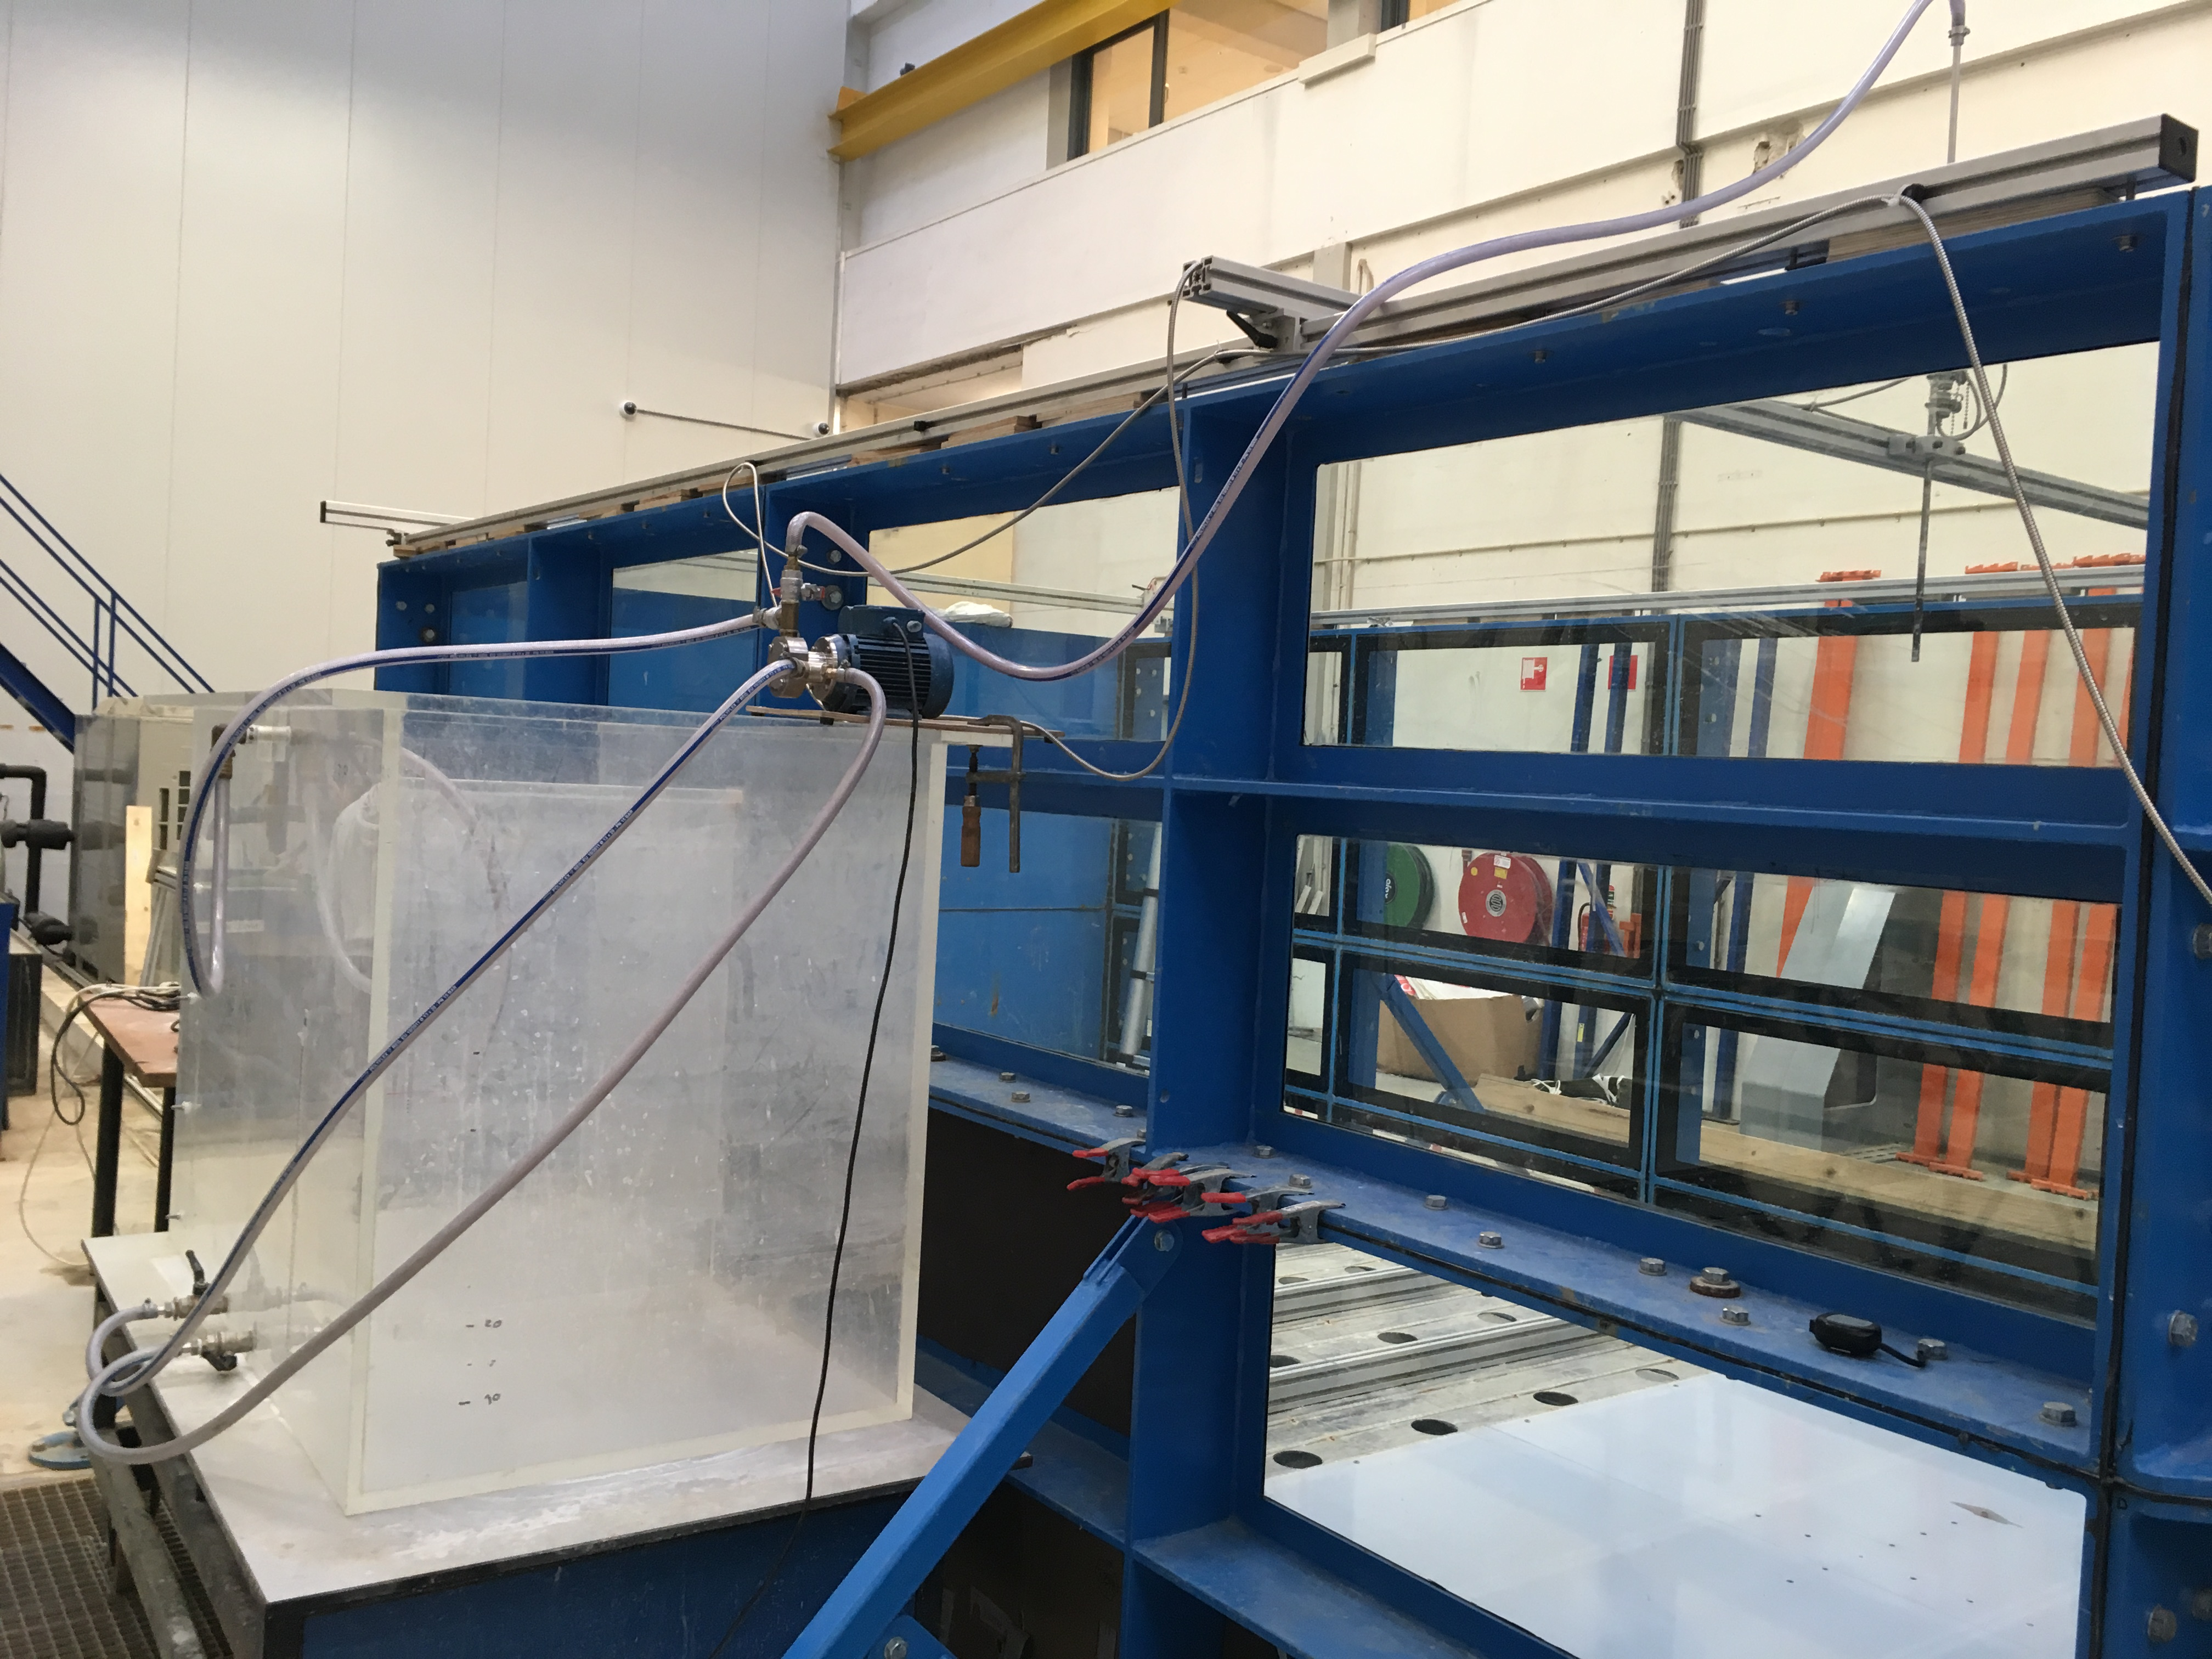
\includegraphics[width=\linewidth]{Images/Mixing_Tank.png}
  \caption{Mixing tank with impellor pump}
  \label{subfig:mixing_tank}
\end{figure}



\newpage
\noindent\textbf{Connection to overflow shapes} \newline
\noindent When the right mixture density is pumped to the reservoir, it goes through the 10mm diameter pipe (outside diameter 12mm). The aim of this experiment is to look at different overflow shapes and therefore three different shapes are tested, which are shown in figure \ref{fig:inner_sizing_overflow}. At the top of the pipe, a valve can regulate the flow to keep it constant (see figure \ref{fig:subshapes}a). 


\begin{figure}[ht!]
    \centering
    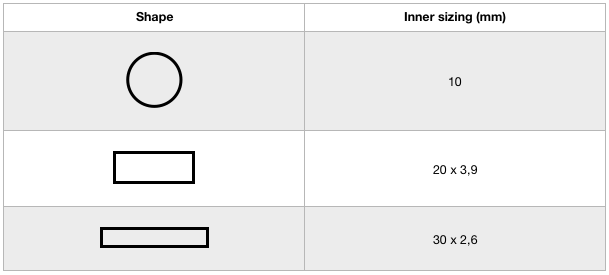
\includegraphics[width=0.6\textwidth]{Images/Inner_sizing_overflow.png}
    \caption{Inner sizing of different shapes needed to maintain same area}
    \label{fig:inner_sizing_overflow}
\end{figure}

%Snelheidsvalve
%verschillene vormen (oppervlakte etc)
%Connectie naar ronde vorm

\newpage
\noindent In order to test different shapes, the inner area is kept the same for all shapes to maintain the same velocity in all cases. From here, the best possible shape can be selected which can be translated to a diffusor. Because the valve is connected to the 12mm round pipe, the chosen option to change the outflow shapes is to slide a different attachment, which contains a part that slides over and a part that changes from a round shape to a rectangular shape,  over the round pipe until a certain point. These attachments are 3D printed in-house of APT Offshore and are shown in figure \ref{fig:subshapes}b. The top parts are the different outflow shapes where the bottom parts are the slip-on parts which slide over the round pipe.


\begin{figure}[ht!]
\centering
\begin{subfigure}{.5\textwidth}
  \centering
  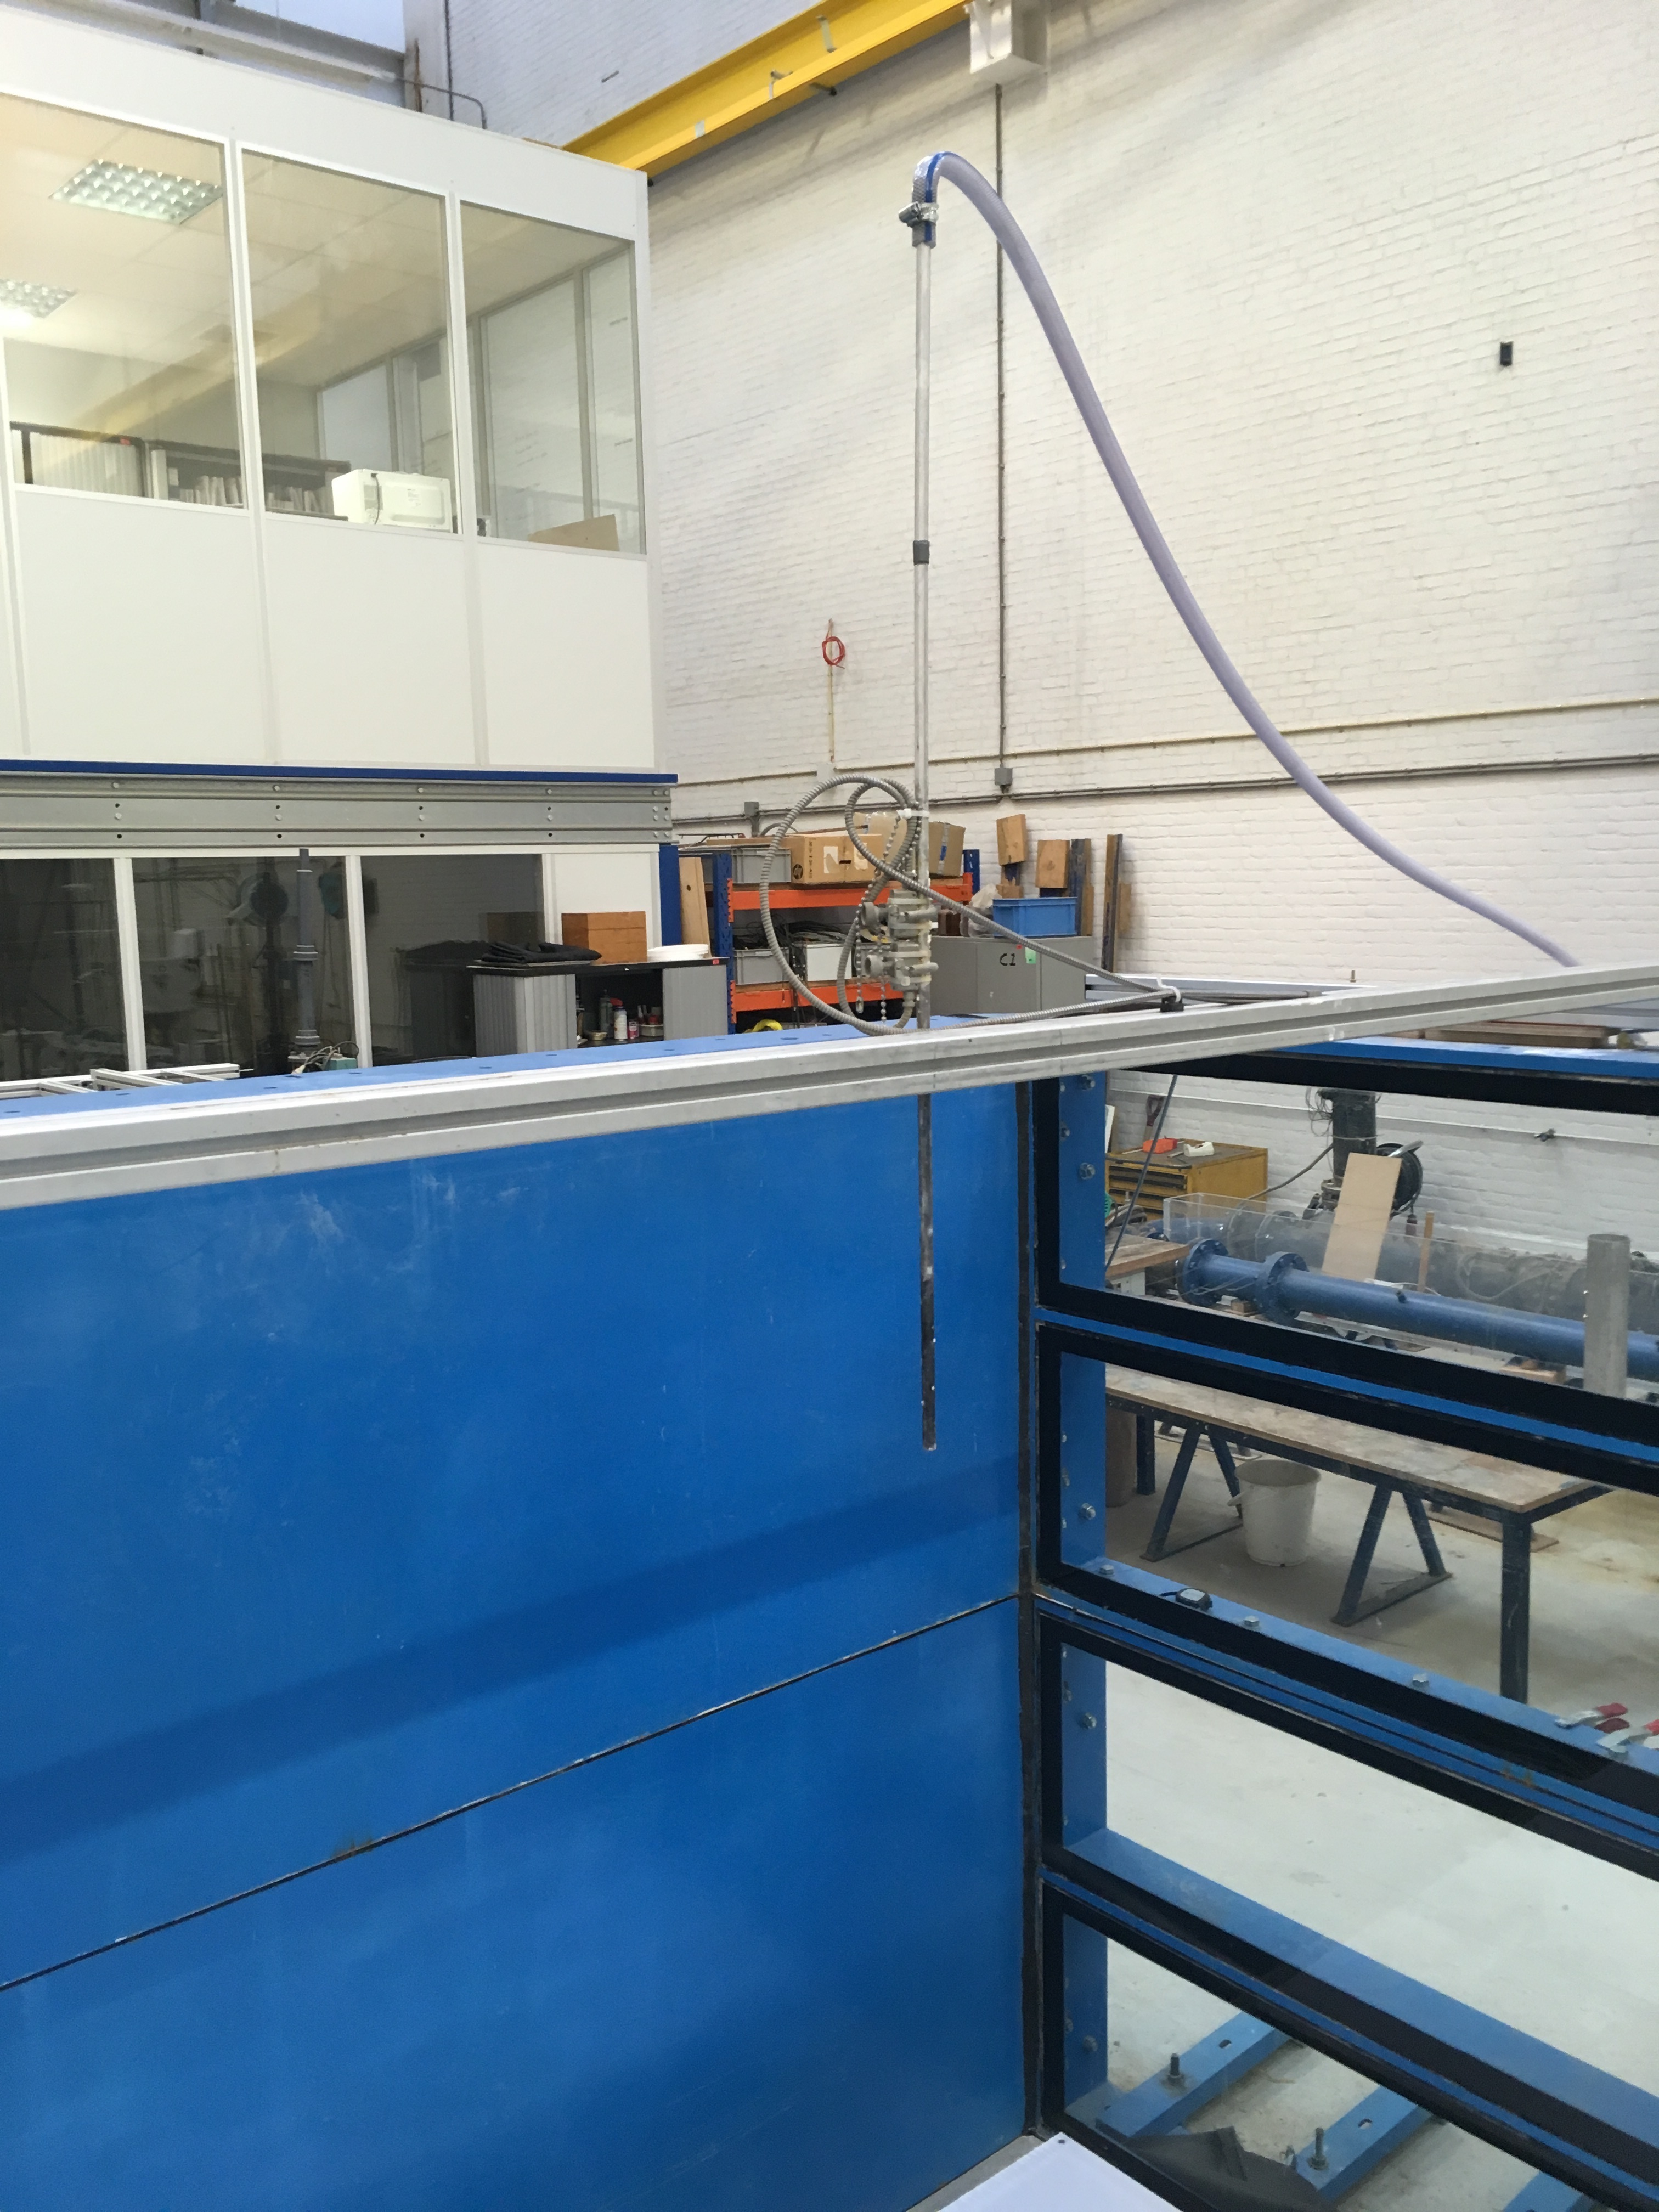
\includegraphics[width=.8\linewidth]{Images/Overflow_test.jpeg}
  \caption{Discharge pipe with valve}
\end{subfigure}%
\begin{subfigure}{.5\textwidth}
  \centering
  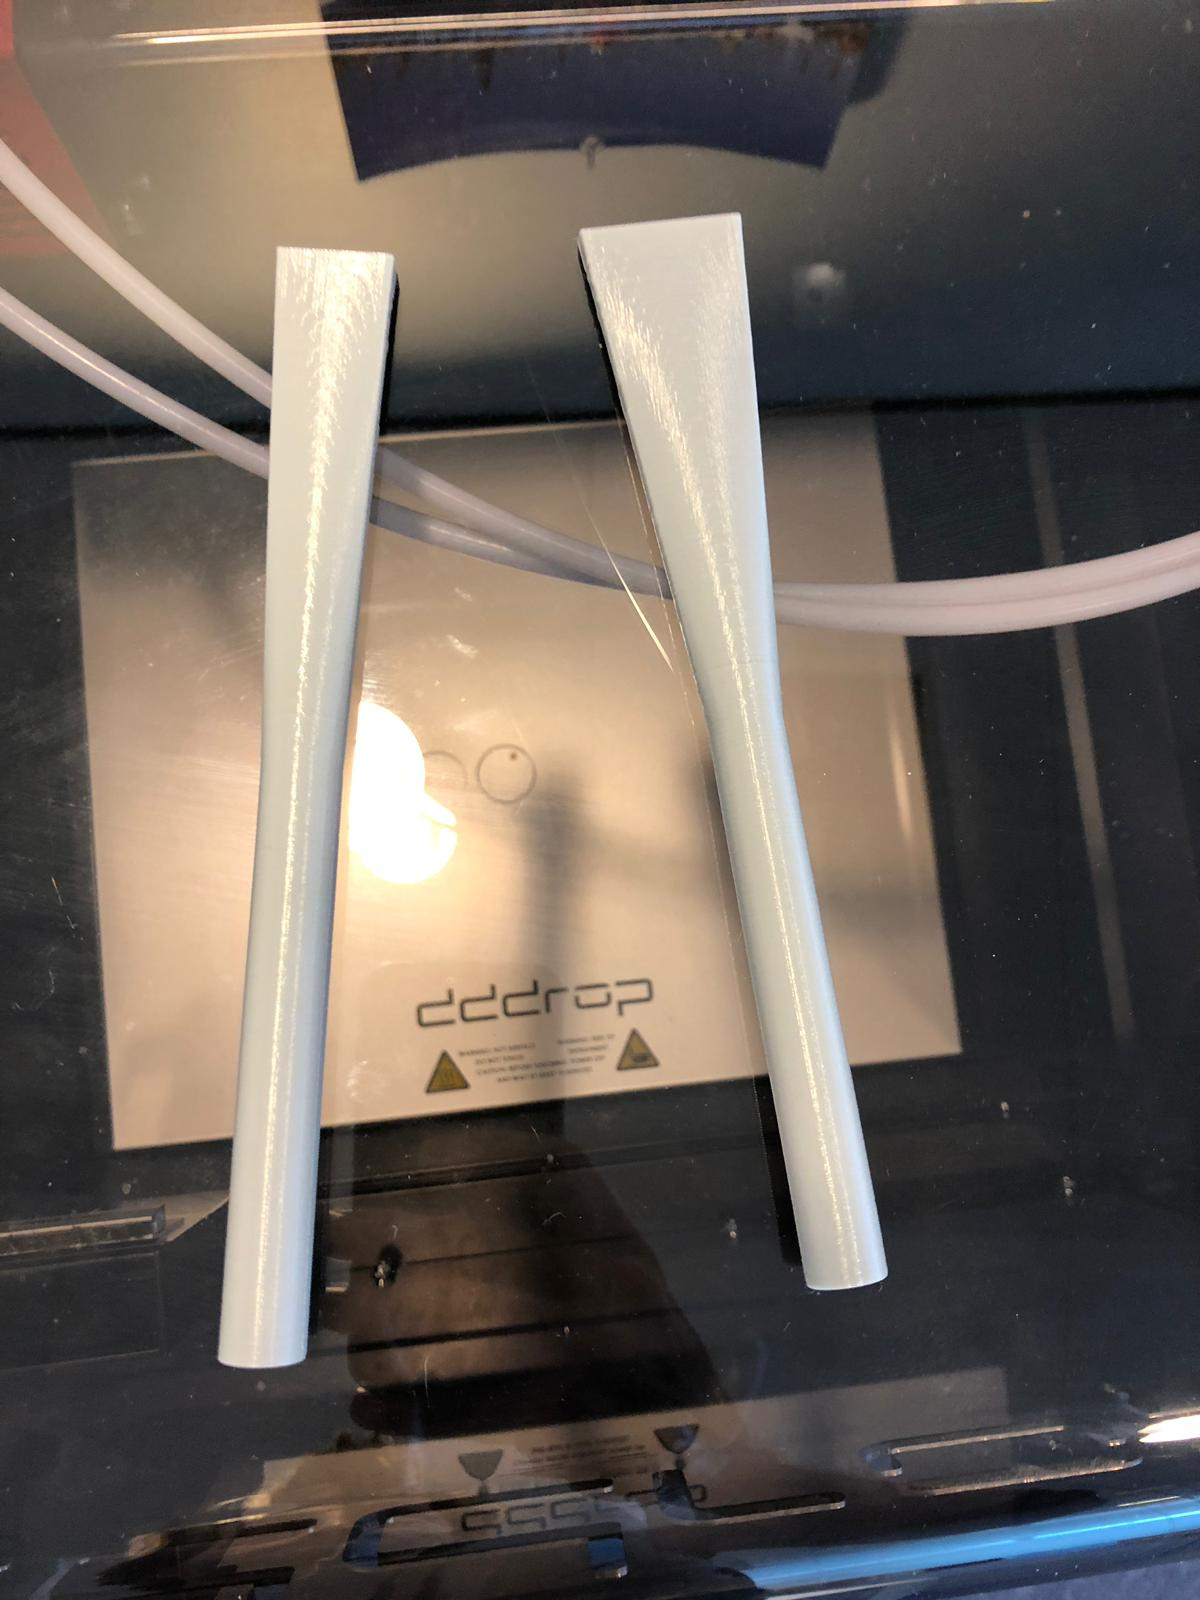
\includegraphics[width=.8\linewidth]{Images/overflow_shapes_3d.png}
  \caption{3D printed overflow shapes}
\end{subfigure}
\caption{}
\label{fig:subshapes}
\end{figure}


\noindent\textbf{Bottom frame} \newline
\noindent When the water-sediment mixture flows into the reservoir trough the round pipe with different shape attachments, it flows into still water where it can spread and fall down on the plate on top of the bottom frame. In this plate, twelve holes are placed in a grid where tubes are connected to twelve valves which all can be opened apart from each other. With these valves, the water sediment mixture from a position in the grid can be sucked up to the drain point where the concentration can be measured. Between the plate and bottom frame are led strips placed for extra light during the tests. An overview of the bottom frame and plate can be seen in figure \ref{fig:frame}.

\begin{figure}[ht!]
\centering
\begin{subfigure}{.66\textwidth}
  \centering
  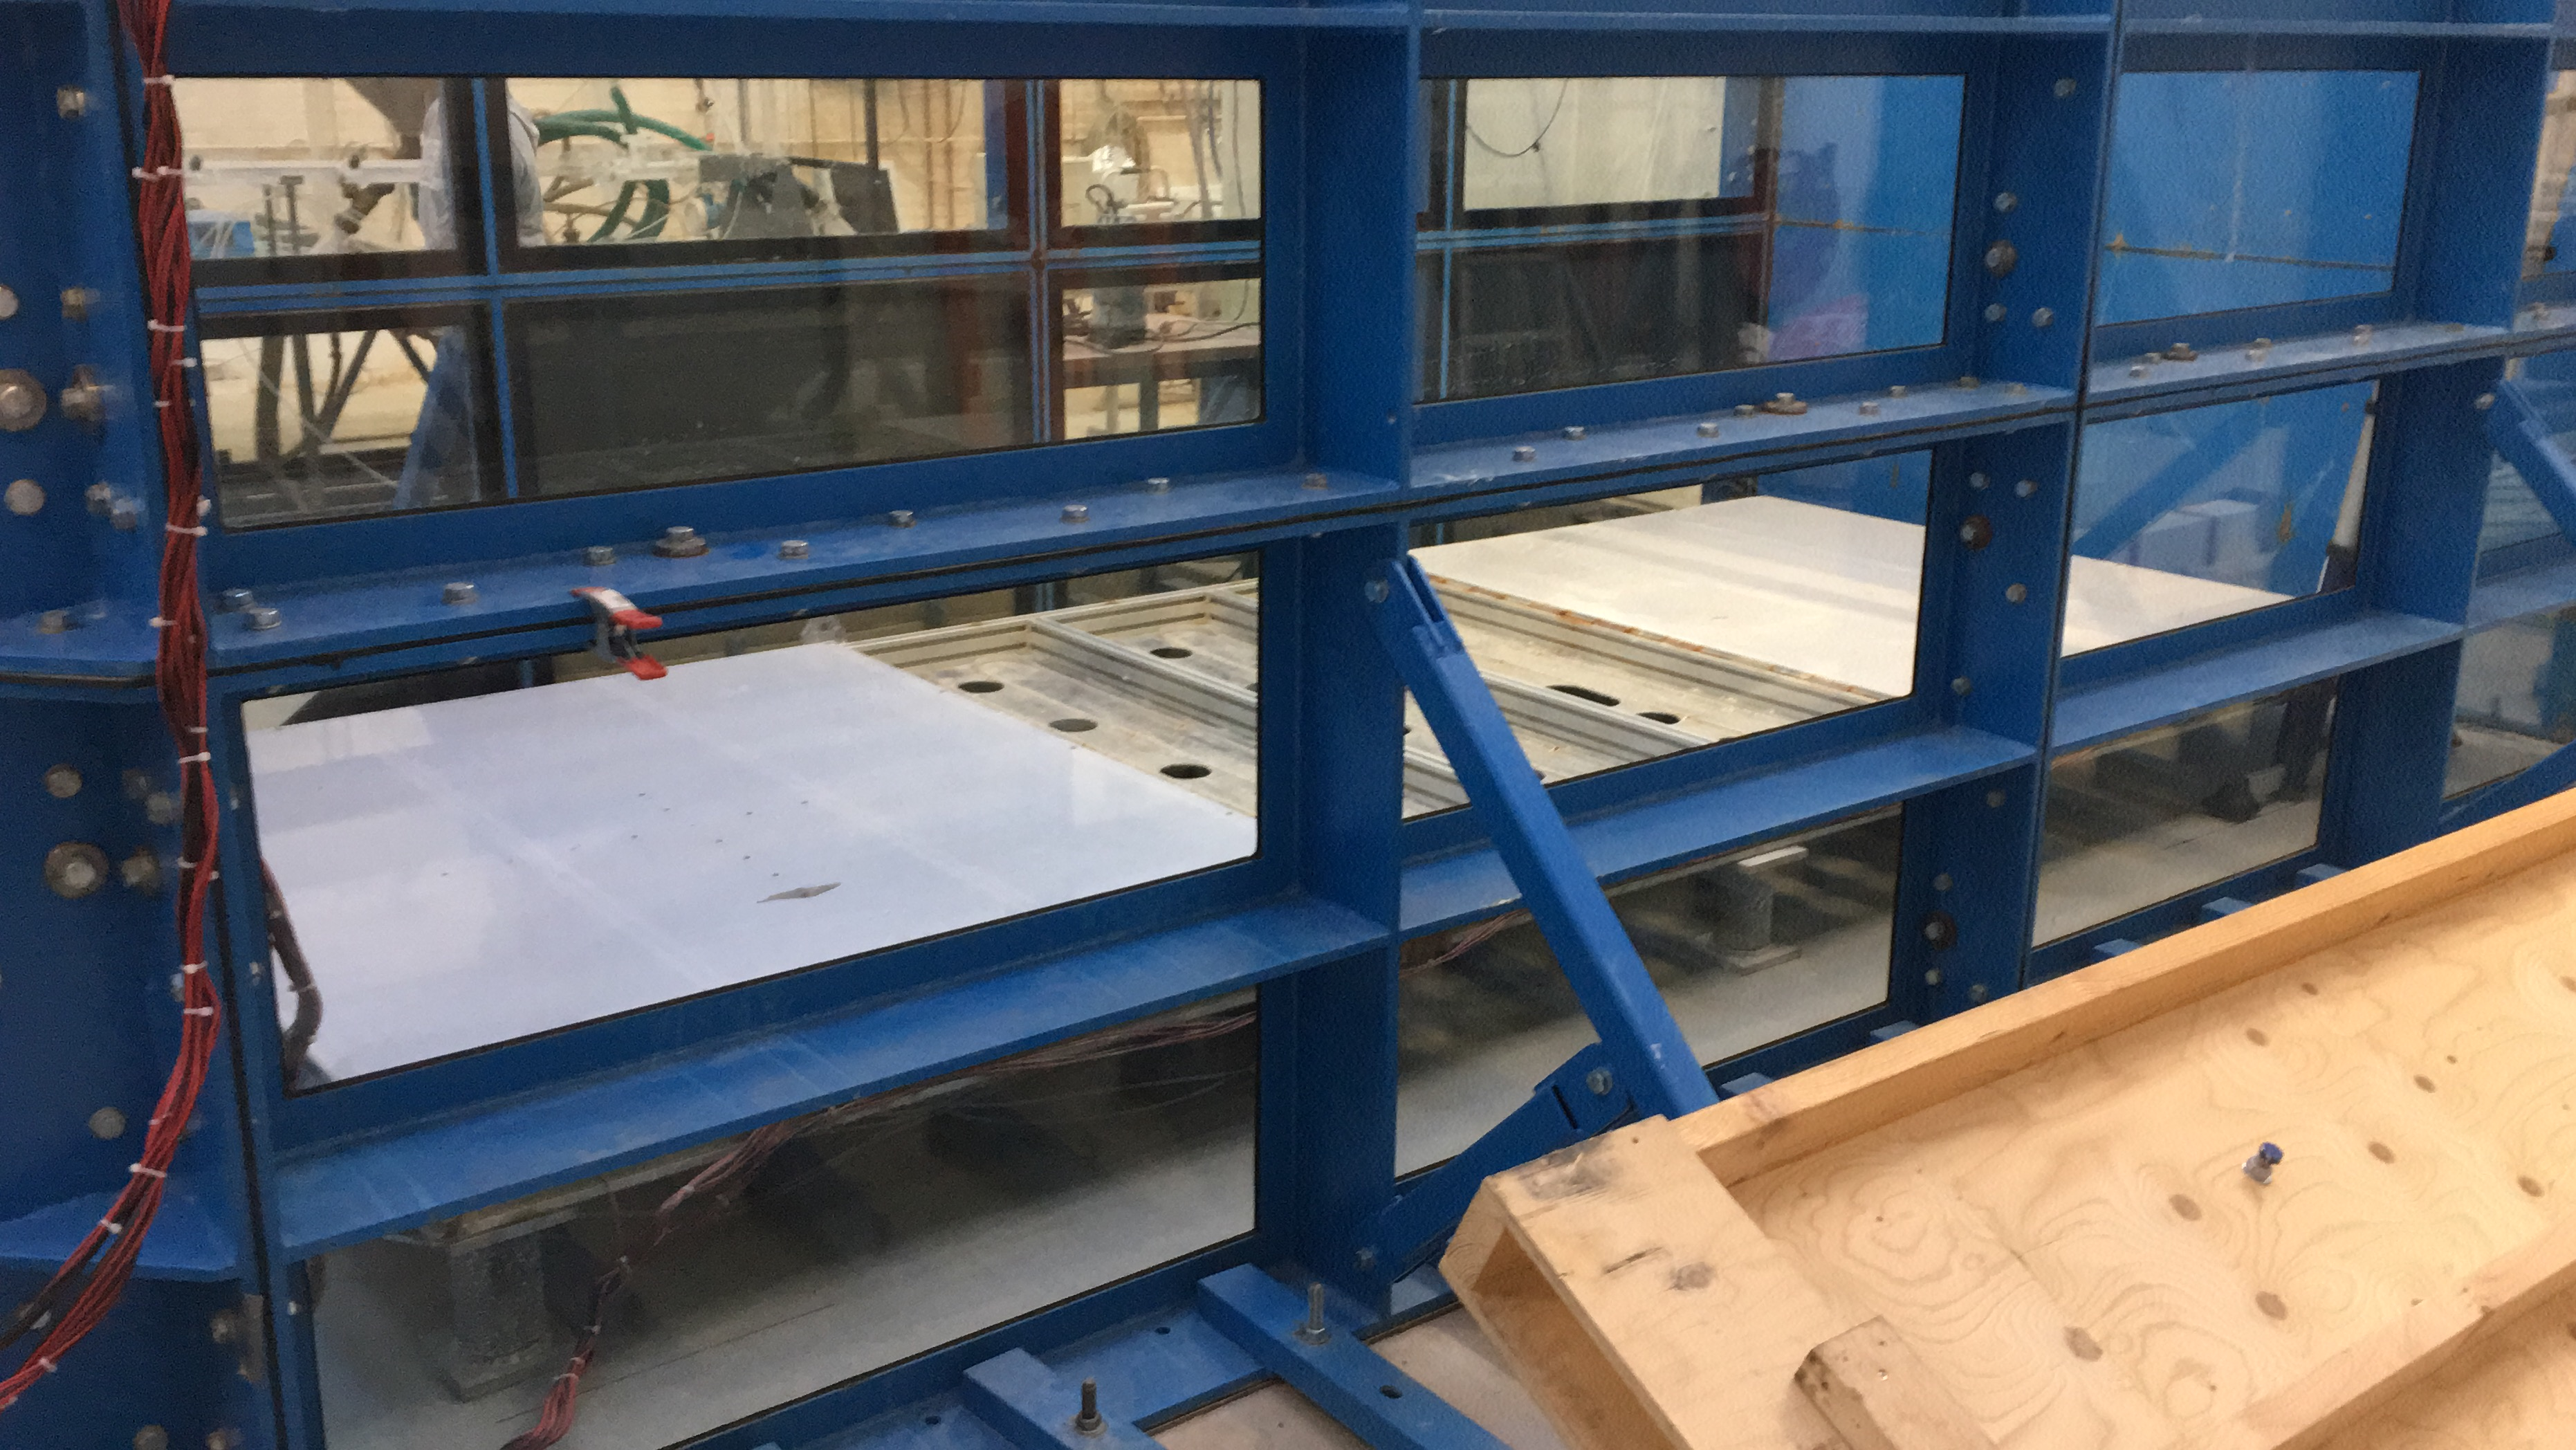
\includegraphics[width=.9\linewidth]{Images/Bottom_frame_test.png}
  \label{subfig:bottom_frame}
\end{subfigure}%
\begin{subfigure}{.34\textwidth}
  \centering
  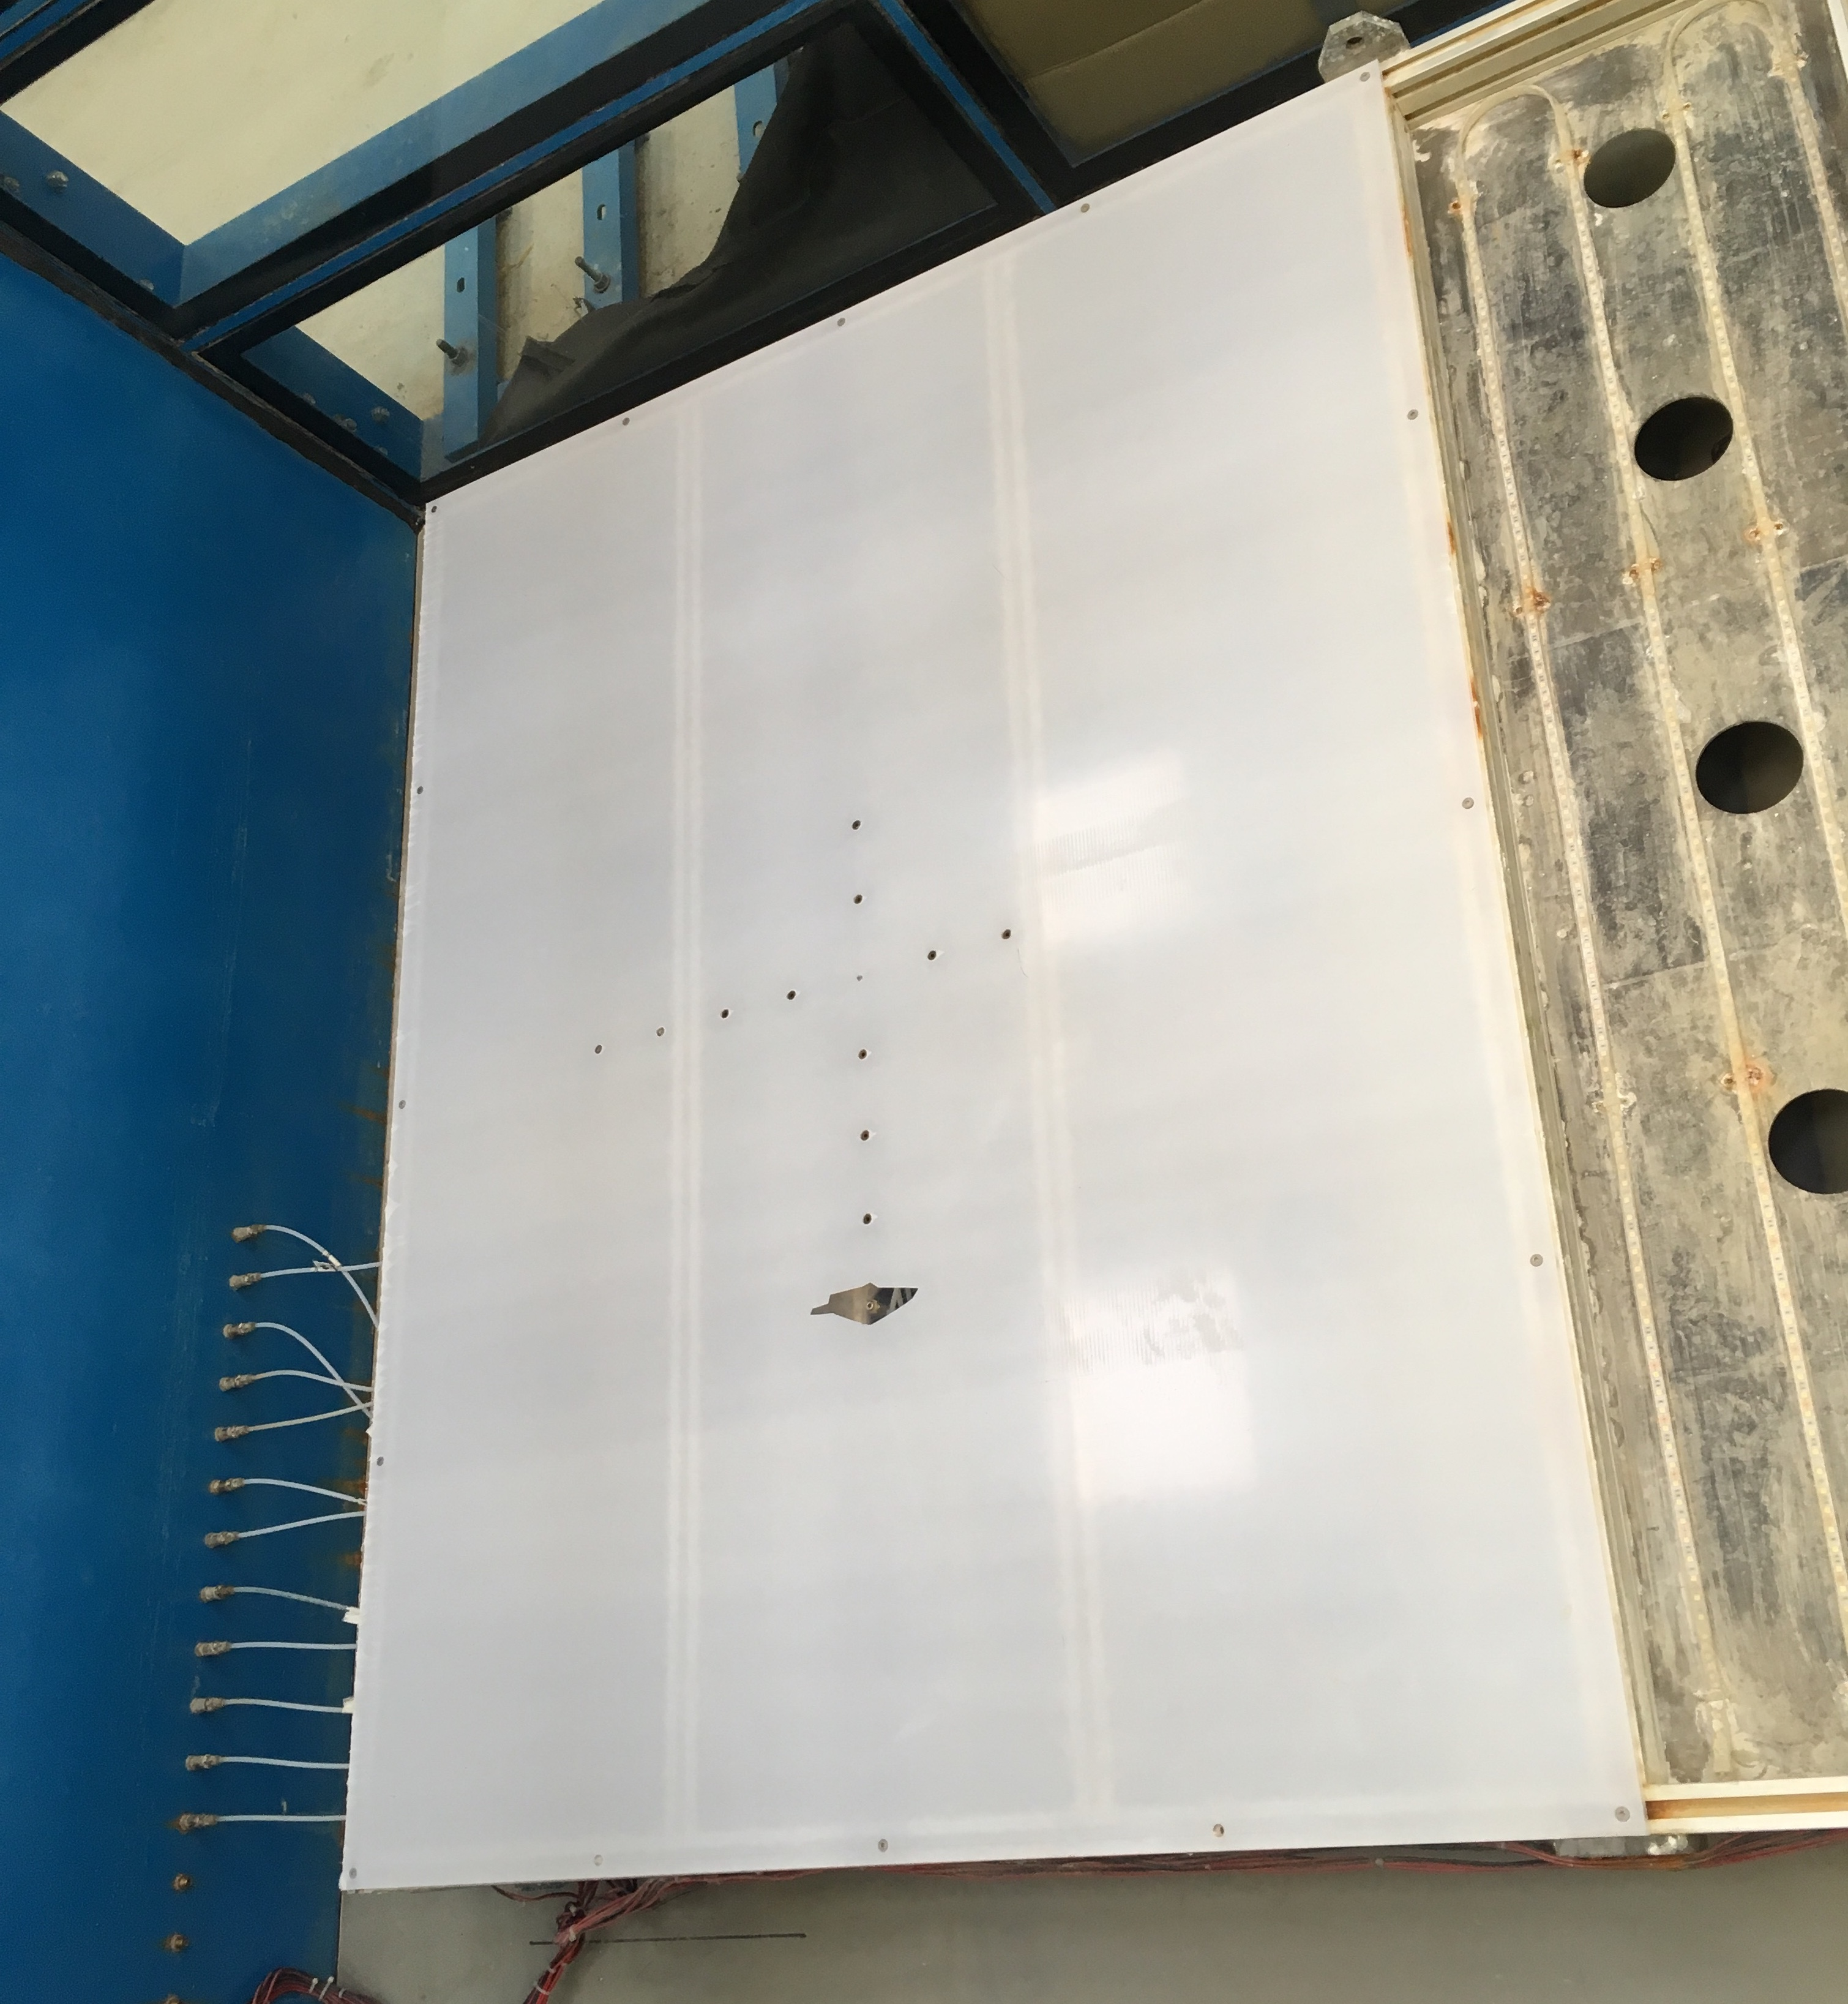
\includegraphics[width=.9\linewidth]{Images/Plate_test.png}
  \label{subfig:plate_test}
\end{subfigure}
\caption{Frame with reservoir and plate with drain points}
\label{fig:frame}
\end{figure}


\section{Experimental parameters}
\label{sec:para}
 


\subsection{Material}
%zeven om hervullen van de tank tegen te gaan met kleine particles
%grain size distribution
As mentioned in chapter 2, due to the slower settling of finer sediment in the hopper with respect to coarser sediment, the overflow and therefore the exiting plume generally contains more mud and finer particles than the dredged material. Therefore a material is chosen which has a particle size distribution comparable to mud, which is quartz powder (figure \ref{fig:quartz_powder}). Quartz powder (20 < d < 90 micron) eases the production of homogeneous mixtures and does not cluster together to form flocs due to its neutral electrical charge. Before use, the quartz powder is sifted to ensure a size of 20 < d < 90 micron. This is done to ensure no blockages of bigger particles inside the discharge pipe.

\begin{figure}[ht!]
    \centering
    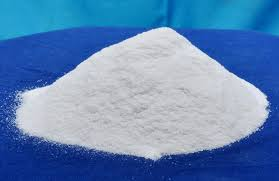
\includegraphics[width=0.5\textwidth]{Images/Quartz_powder.jpg}
    \caption{Quartz powder which is used during the experiments as material}
    \label{fig:quartz_powder}
\end{figure}



\subsection{Discharge}
In order to create a turbulent plume, a Reynolds value of > 2000 should be considered. Combining this with a discharge diameter of 10mm, the flow velocity of the mixture should be > 0.2m/s. In order to have some tolerance, it is chosen to have a outflow velocity of 0.35 m/s. It should be noted that the quartz powder particles will increase turbulence with the same Reynolds number comparing with normal tap water. Also the height in the tank is limited and therefore a lower outflow velocity means less interaction with the bottom plate. Interaction with the bottom plate will cause re-suspension of the material which simulates a seabed. This effect is not desirable in the experiment and so the height is maximized (1.585m) and outflow velocity is minimum to maintain a turbulent plume (0.3 m/s). \newline
\noindent To achieve a stable outflow velocity, the discharge flowrate is regulated by the jet valve with the help of a flow meter (Katronic KATflow 200). KATflow (figure \ref{fig:Katronic}) is a portable instrument with two transducers fixed on the pipe wall. The key working principle of the instrument is that sound waves traveling with the flow will move faster than those traveling against it. Hence, the difference in the transit time of these signals is proportional to the flow velocity of the liquid and consequently the flow rate. Before the use, the instrument needs to be set and adjusted to the pipe and flow characteristics. For the instrument calibration, a known volume of the mixture is pumped over a fixed time and compared with the instrument output registered flow volume. 

\begin{figure}
    \centering
    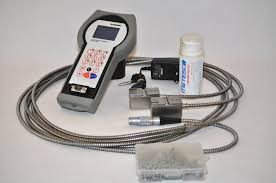
\includegraphics[width=0.3\textwidth]{Images/Katronic.jpg}
    \caption{Katronic KATflow 200 instrument used to set right flow discharge}
    \label{fig:Katronic}
\end{figure}

\noindent It is advantageous to use the KATflow, as the instrument displays the instantaneous flow velocity or flow rate, which gave a possibility to set the flow before the start of the tests. Also, in case of changes in the flow rate, it is possible to quickly stabilize the flow to the required discharge velocity by turning the ball valve between the pump and the jet pipe.

\subsection{Mixture density}
In the mixing tank, tap water is mixed with quartz powder to create a certain mixture density. First of all the visibility is important for the video imaging. Previous tests done in the reservoir by \cite{Warringa} and \cite{Byishimo} used the same experimental setup. Both users compared three different mixtures (5,10,20 gram quartz powder / liter water) in their experiments. Visibility in all cases was not a problem. It should be noted that both experiments looked at impact on the seabed during deep mining operations. Because interaction with the bed leads to re-suspension of the material which is not desired in this experiment, the mixture density is chosen by looking at the re-suspension in the experiments of \cite{Warringa}. \cite{Warringa} compared three heights (0.25, 0.5, 1m). Because the height in this experiment is maximized (1.5m) an overview is shown in figure \ref{fig:Warringa_gl} containing all different mixture densities at height 1m.

\begin{figure}[ht!]
    \centering
    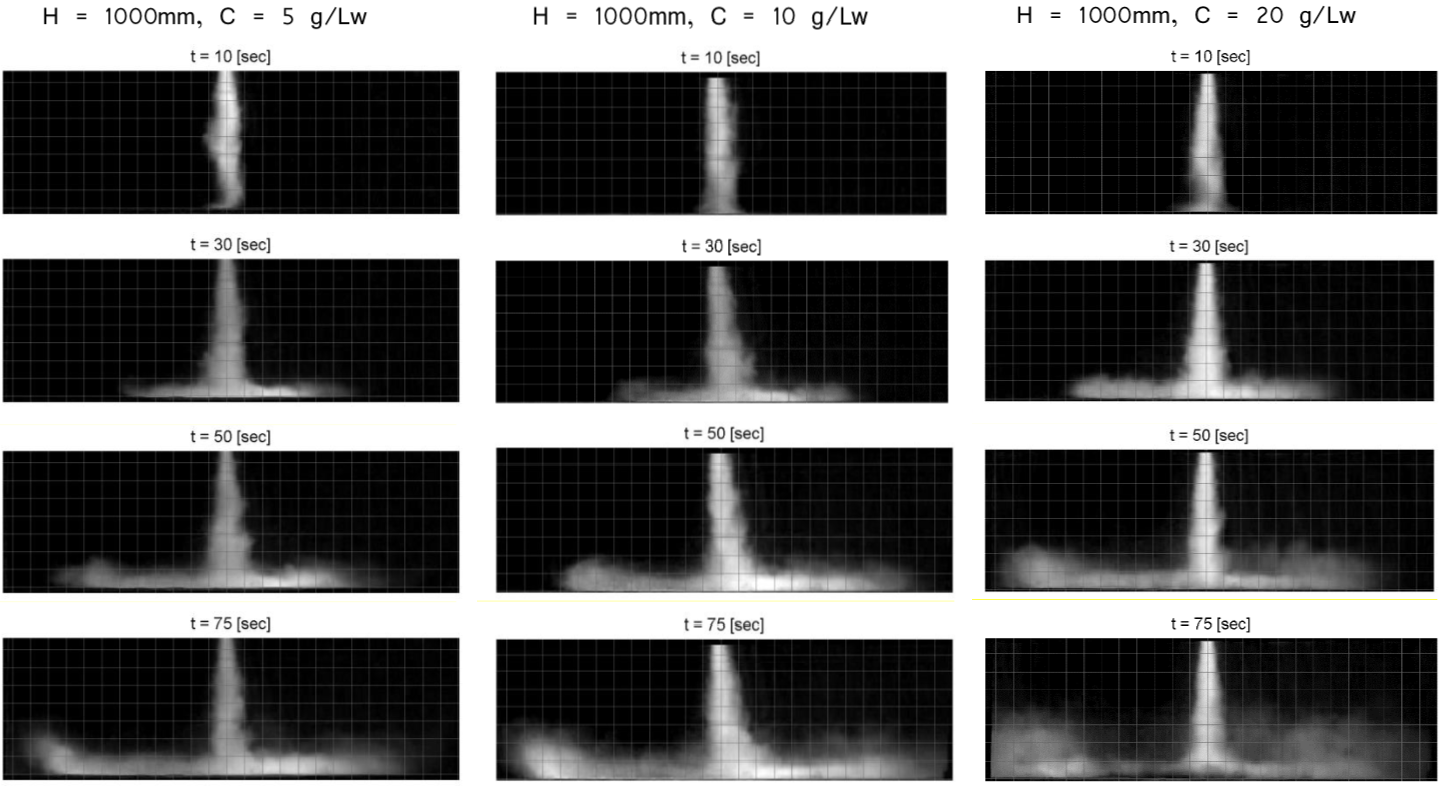
\includegraphics[width=1\textwidth]{Images/Warringa_gl.png}
    \caption{Comparison of re-suspension due to the bottom plate between three densities in experiment of \cite{Warringa}}
    \label{fig:Warringa_gl}
\end{figure}


\noindent Looking at figure \ref{fig:Warringa_gl}, it can be seen that the mixture with a suspended sediment concentration of 20 g/l has the most re-suspension due to interaction with the bottom plate. Between a SSC of 5 g/l and 10 g/l shows not much difference in re-suspension height but does in re-suspension density. It should be noted that quartz powder has a polishing effect on the impellor pump which will damage it over time. Due to this, adding more quartz powder will assure more damage to the impellor pump. Due to this, a SSC of 5 g/l is chosen to use during the experiments. Also it should be noted that mixture density has influence on the plume angle and so the entrainment factor.  \newline

\noindent \textbf{Water Temperature} \newline
To ensure no extra density differences due to difference in temperature between the water in the reservoir and in the mixing tank, the temperature of the reservoir is measured before each test. This temperature is set to be maintained inside the mixing tank within a range of 0.3 degrees below or above, because during experiment, the water in the mixing tank warms up with roughly an amount of 0.3 degrees. Adding warm water or use the submersible pump will increase the water temperature, cooling can be done by ice in closed bag or with tap water and adding sediment to keep a constant concentration.




\newpage
\section{Obtainment data}
\subsection{Suspended concentration}

To measure the concentration of suspended particles in the plume, local SSC samples are taken by tubes installed in the table, which connects to drain points on the outside of the reservoir. The samples are measured with a high accuracy laboratory Turbidity meter AL450T-IR by which turbidity values were obtained as NTU value. A picture of it is shown in figure \ref{fig:turbiditymeter}.

\begin{figure}[ht!]
    \centering
    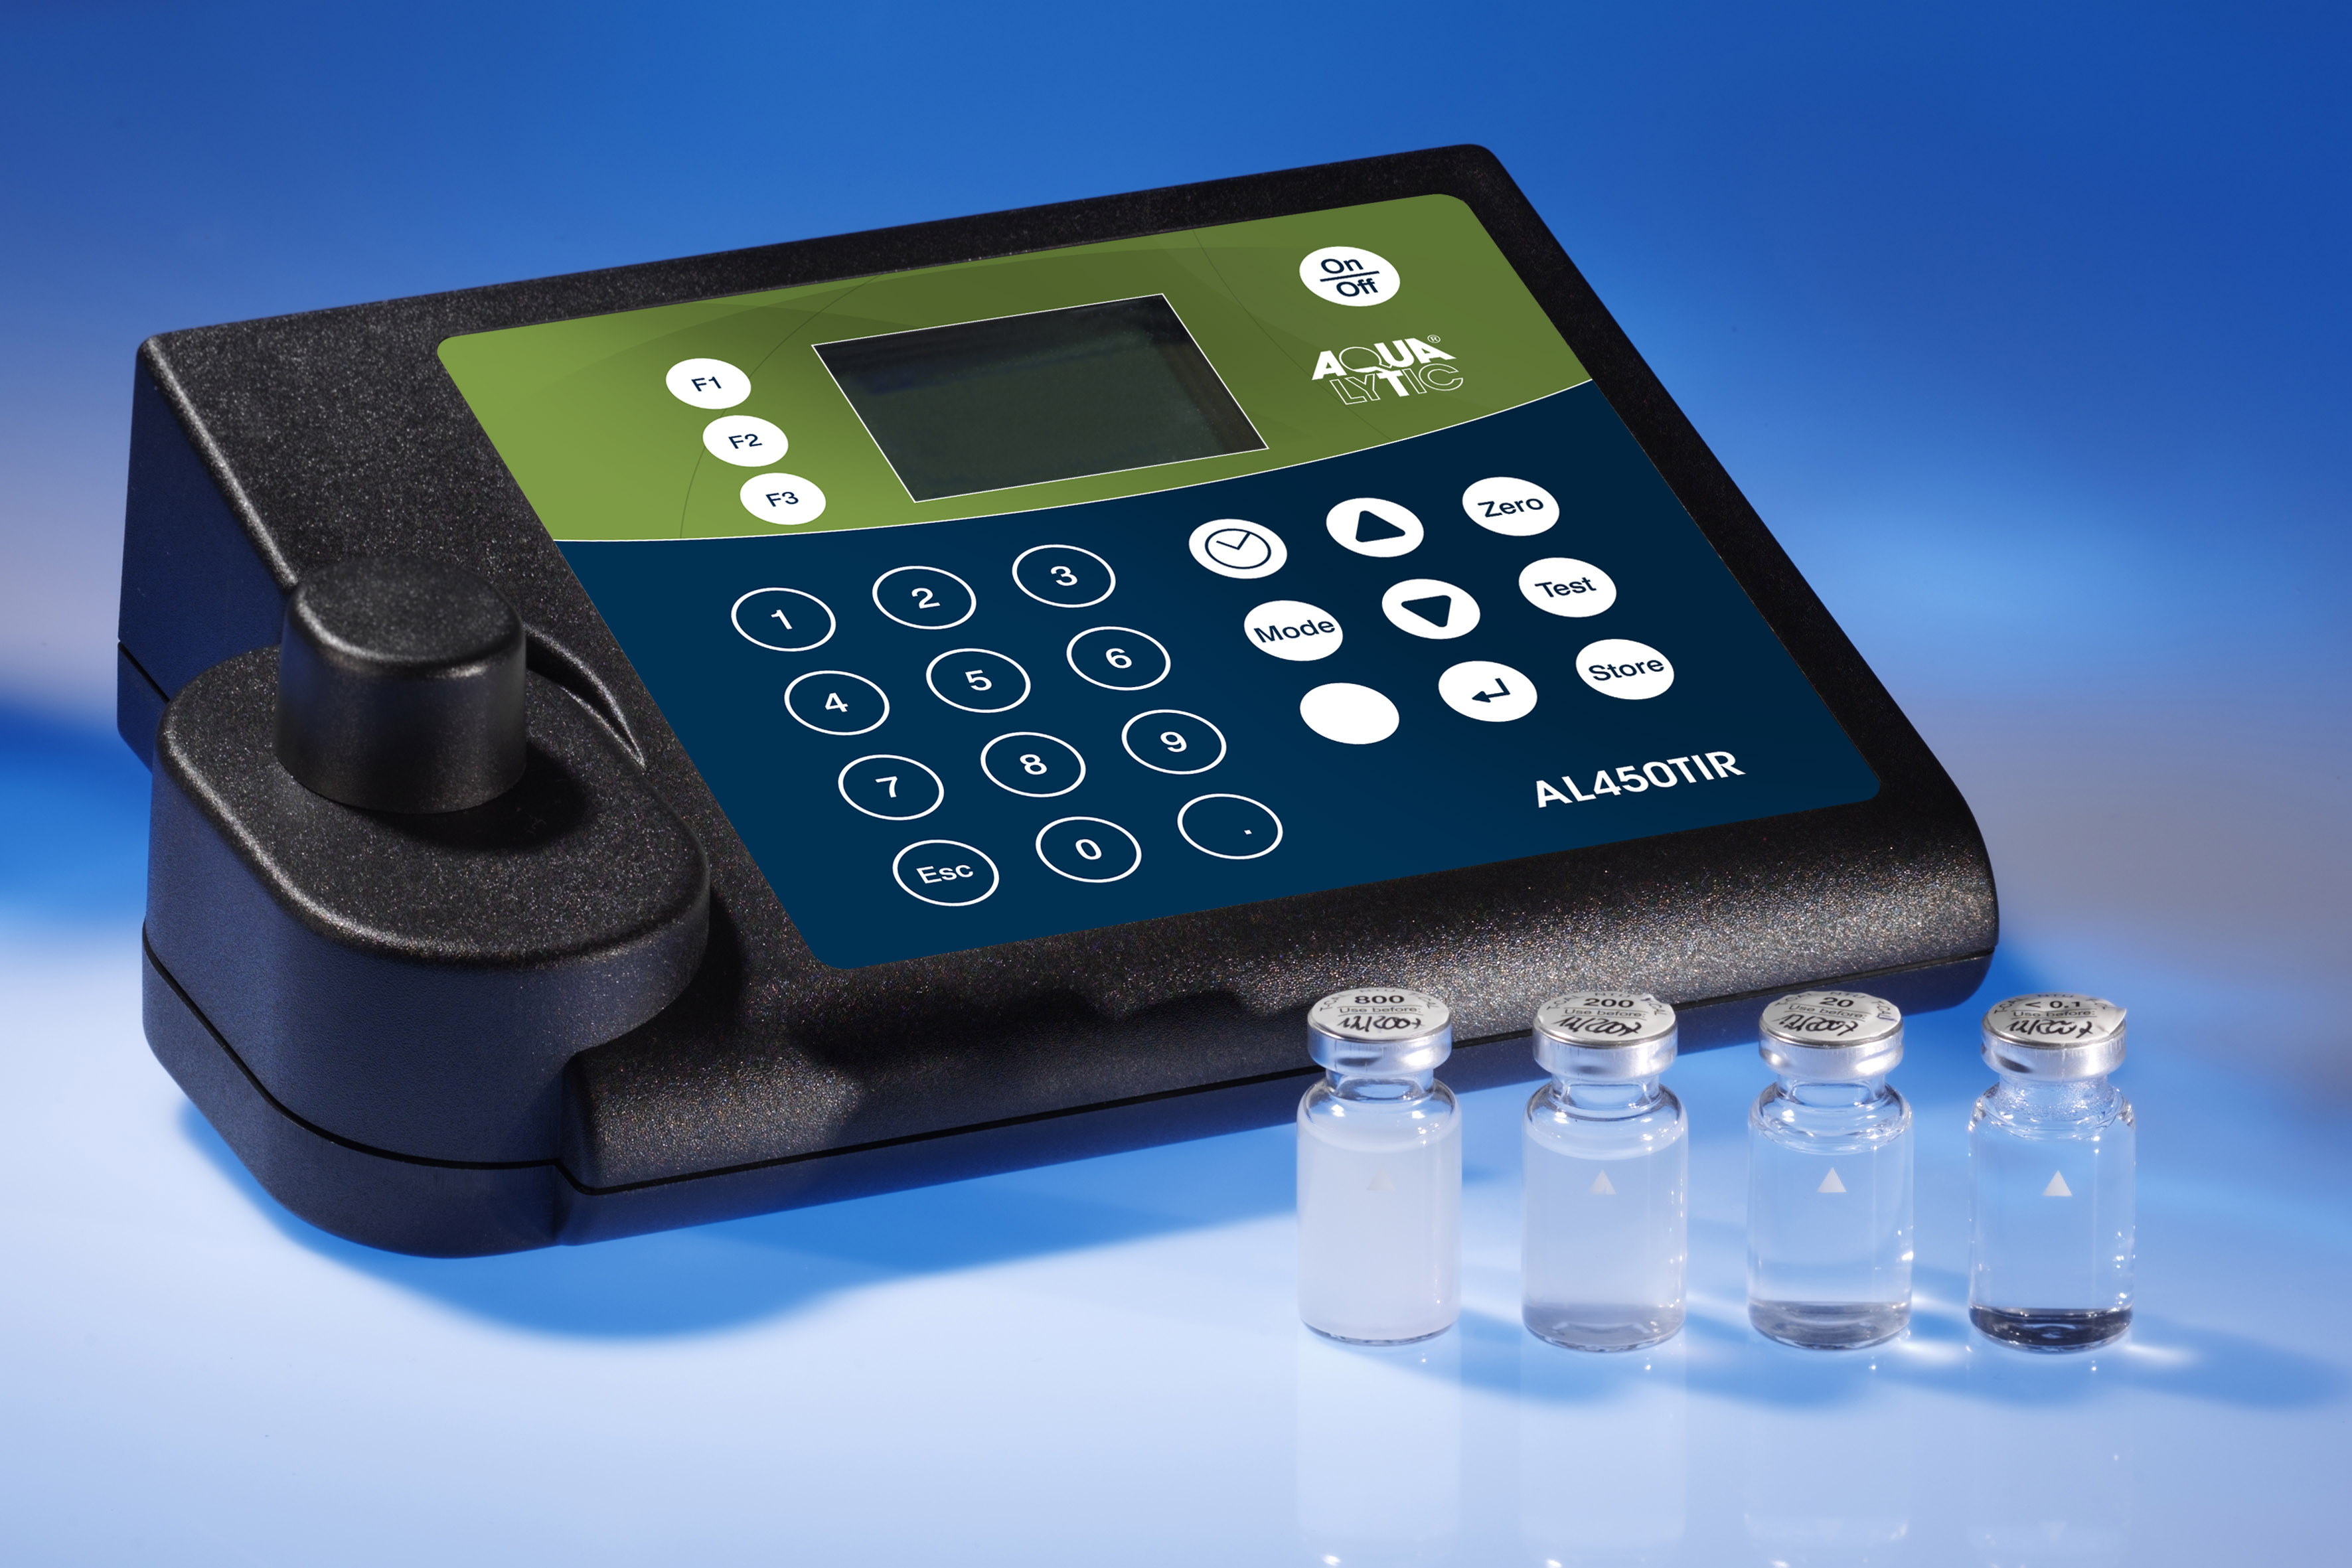
\includegraphics[width=0.3\textwidth]{Images/al450_tir.jpg}
    \caption{Aqualytic Turbidity meter AL450TR-IR}
    \label{fig:turbiditymeter}
\end{figure}


\noindent The turbidity meter AL450T-IR is an optical portable turbidity meter designed with the requirements of ISO 7027, for the determination of turbidity for water quality with a measurement auto ranging over the range of 0.01 to 1100 NTU. The operating principles are based on positioning a transparent vial filled with the sample inside the instrument sample chamber. When the measuring button is pressed, an infrared LED (light emitting diode) with a wavelength of 860nm is emitted immediately. The emitted light is reflected by turbidity in the sample. The scattered light will be detected at an angle of 90° by a photo diode.\newline
\noindent As an output, the sensor will show on the screen the NTU value. In order to minimize errors, the vials and caps should be cleaned inside and outside thoroughly after each test to avoid interference's. The outside of the vial must be clean, dry and wiped with a smooth cloth to remove fingerprints, dust or water drops. Details of the working principle of Turbidimeter AL450T-IR can be found on the manufacturer website. \citep{website:Turbidity} \newline
\noindent After an experiment is started and a steady state is reached; one by one, the tube end valves are flushed for 30 seconds in order to clean them. Previous experiments of \cite{Byishimo} showed that steady state differs for each measuring point, in other words, the distance of the measuring point with respect to the impingement point. Steady state increases with distance so the outer measurement points will occur a later steady state. In order to minimize wall effects and so resuspension of the plume, the outer measurement points are tapped first after they reach a steady state. It is fair to say that the time it takes of the plume to reach a measuring point and multiple that by two, a steady state is reaches \citep{Byishimo}. This time was measured by eye and was approximately 85 seconds. A time of 180 seconds is so fair to begin tapping the outer measurement points. When the tube is cleaned, samples are taken for each point on the measurement map shown in figure \ref{fig:plaat_meetpunten}. The process of taking a a good sample are shown in an overview in figure \ref{fig:NTU_steps}.


\begin{figure}[ht!]
    \centering
    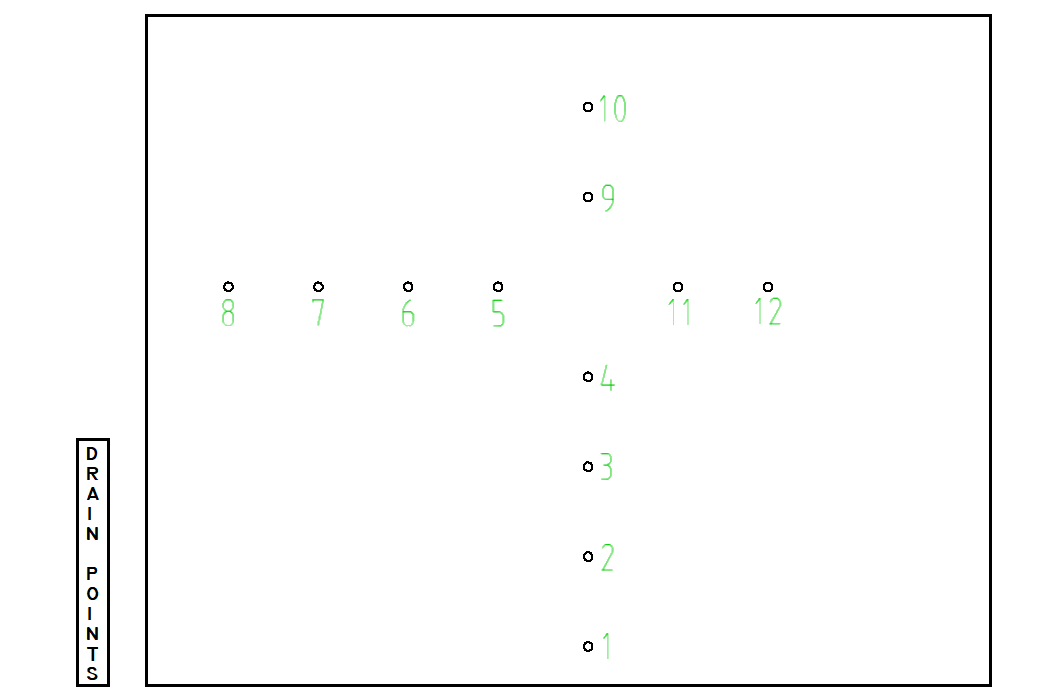
\includegraphics[width=0.6\textwidth]{Images/meetpunten.png}
    \caption{Measurement map plate (top view) with placing drain points. Also see figure \ref{fig:frame}}
    \label{fig:plaat_meetpunten}
\end{figure}

\begin{figure}[ht!]
\centering
\begin{subfigure}{.14\textwidth}
  \centering
  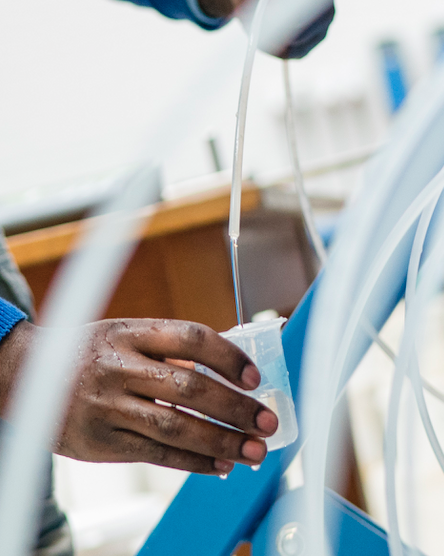
\includegraphics[width=.9\linewidth]{Images/Sample_1.png}
  \subcaption{drain sample}
\end{subfigure}
\begin{subfigure}{.149\textwidth}
  \centering
  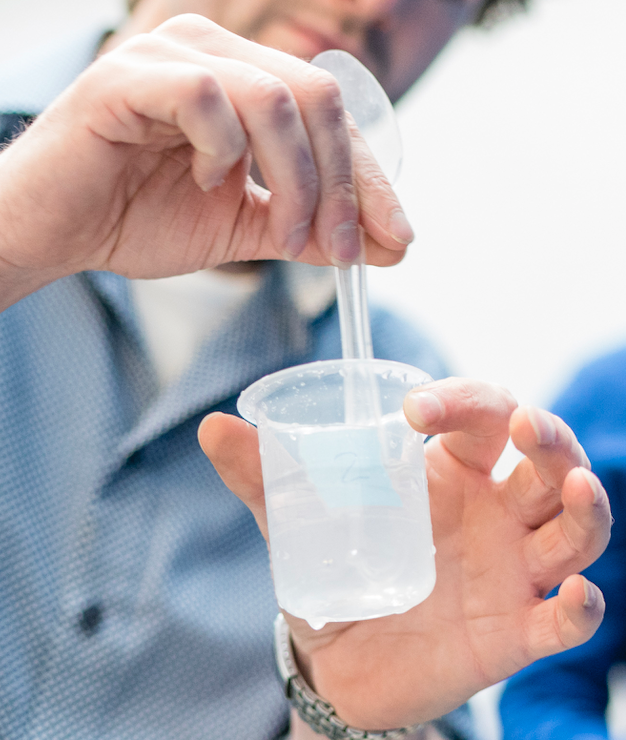
\includegraphics[width=.9\linewidth]{Images/Sample_2.png}
  \subcaption{mix}
\end{subfigure}
\begin{subfigure}{.282\textwidth}
  \centering
  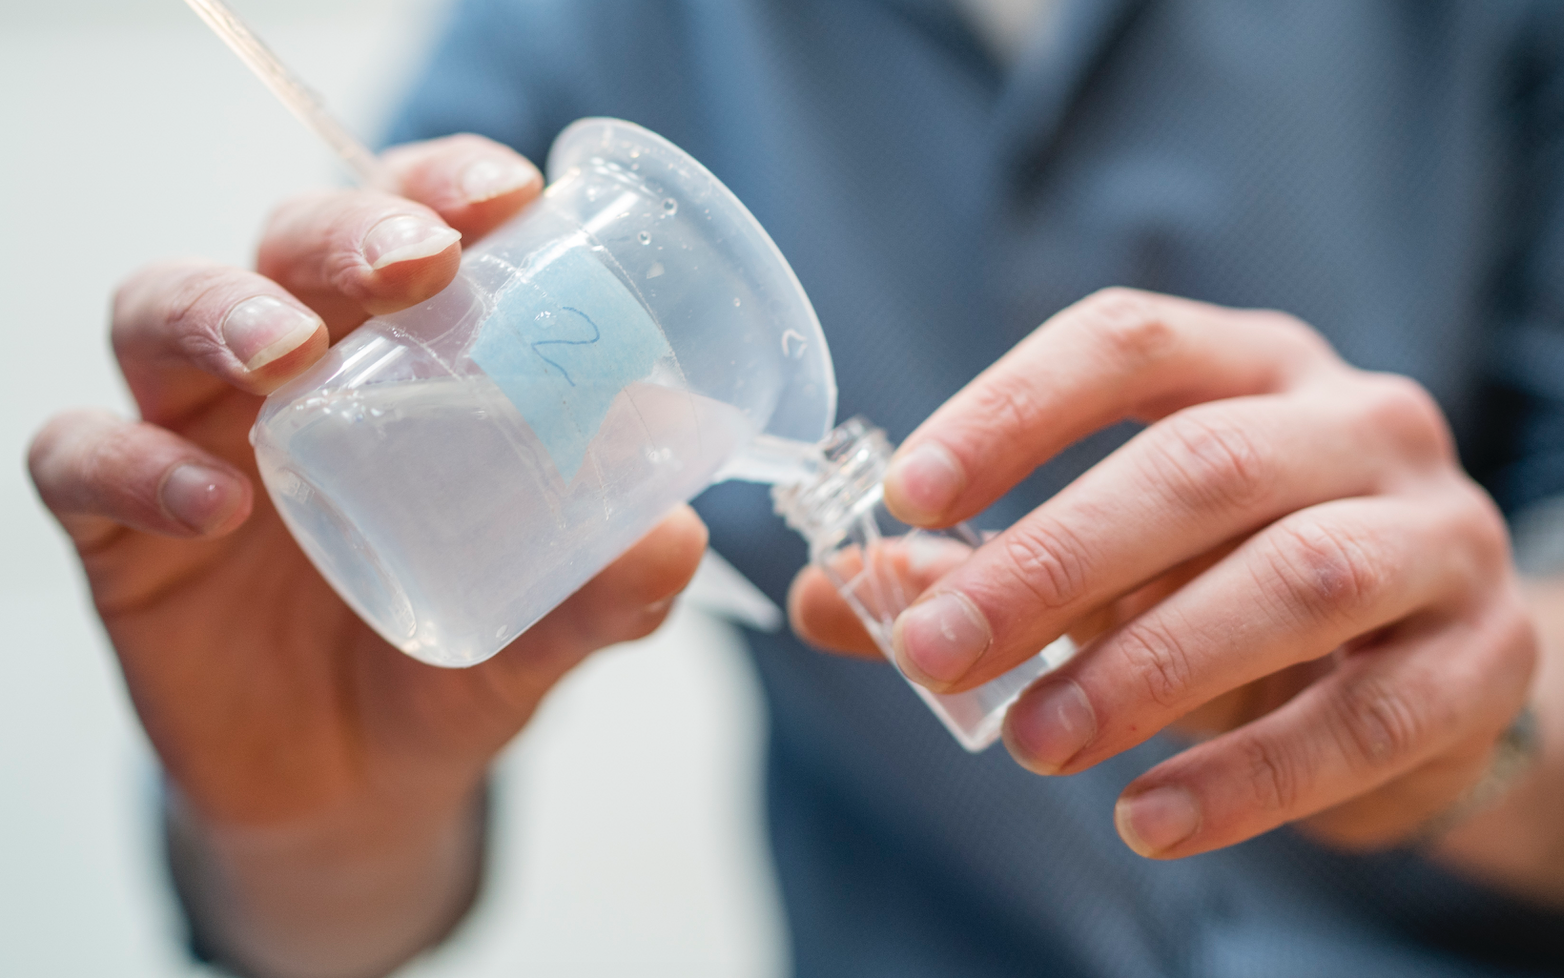
\includegraphics[width=.9\linewidth]{Images/Sample_3.png}
  \subcaption{pour in vial}
\end{subfigure}
\begin{subfigure}{.164\textwidth}
  \centering
  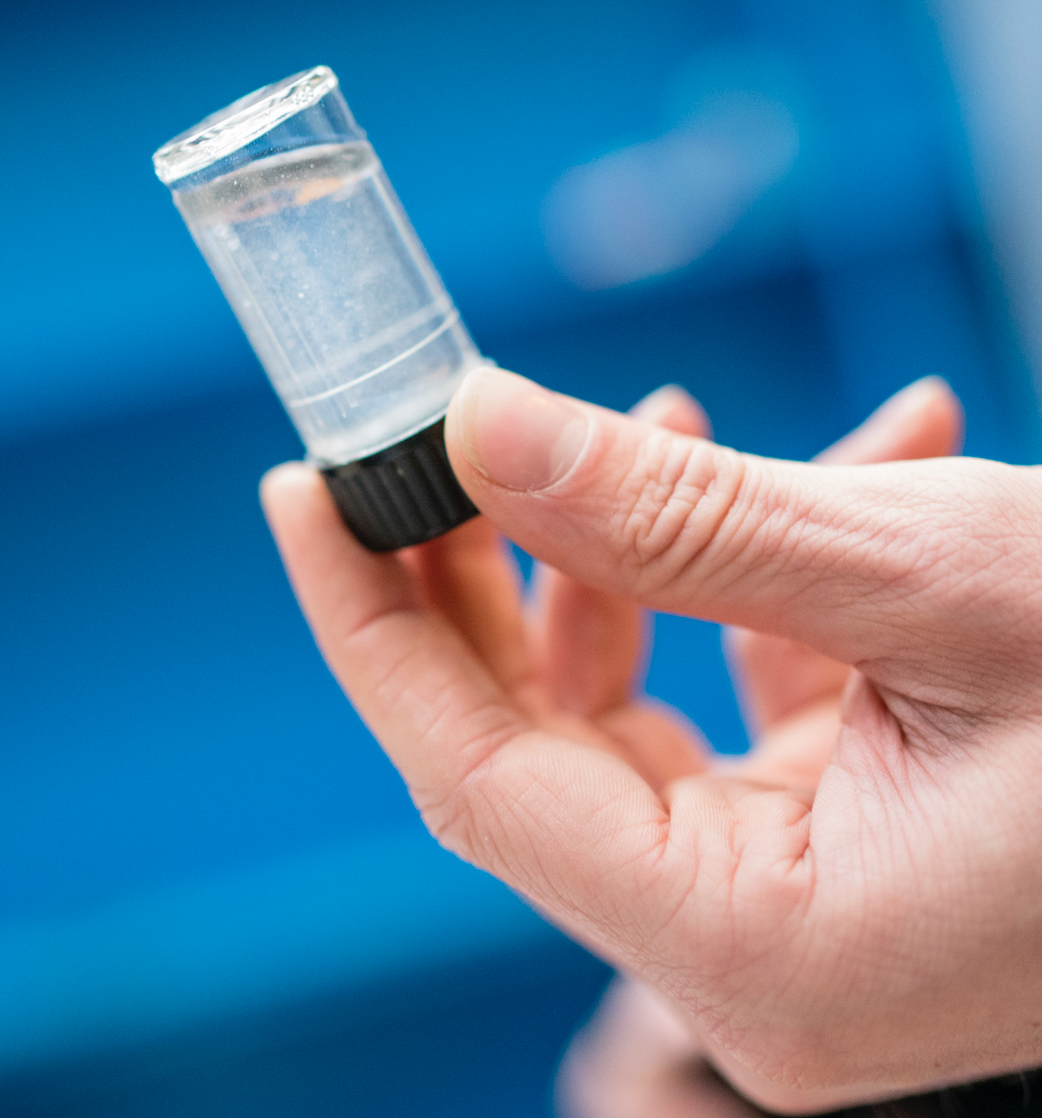
\includegraphics[width=.9\linewidth]{Images/Sample_4.png}
  \subcaption{vial mixing}
\end{subfigure}
\begin{subfigure}{.202\textwidth}
  \centering
  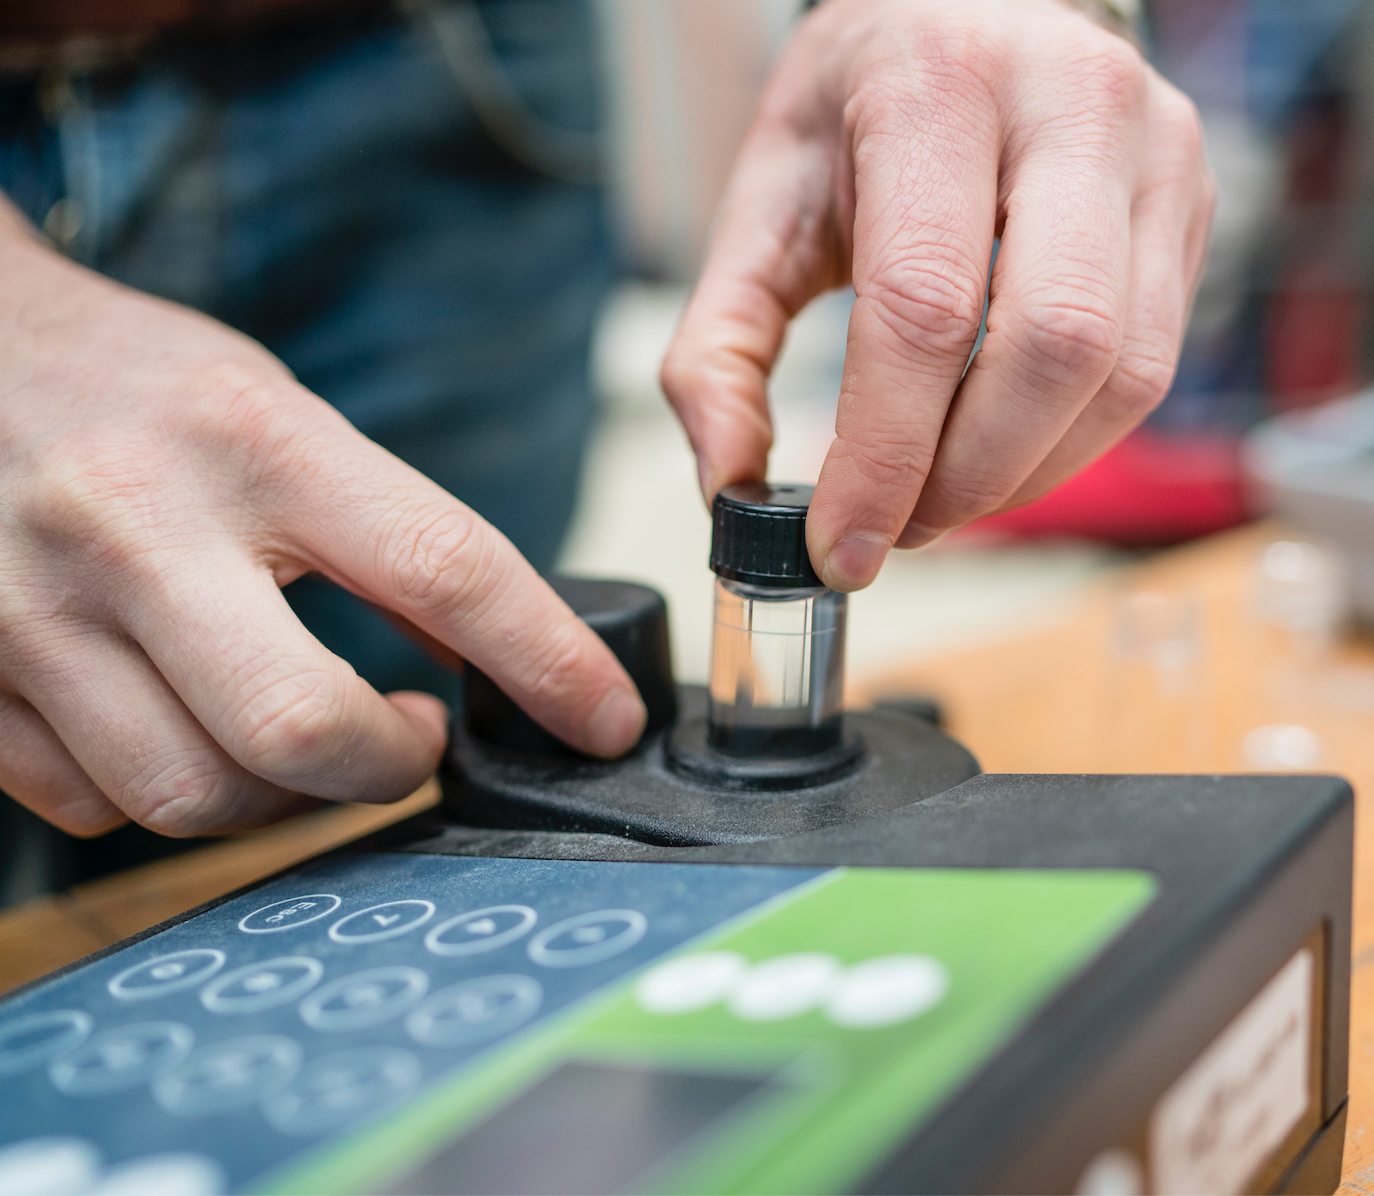
\includegraphics[width=.9\linewidth]{Images/Sample_5.png}
  \subcaption{NTU measuring}
\end{subfigure}
\caption{Steps for sample Turbidimeter (Pictures: Ivo Par)}
\label{fig:NTU_steps}
\end{figure}



\noindent Turbidity measurements are called local and near-bed SSC measurements because in the experiments of \cite{Byishimo} it was noticed that not only the water at the table surface was drained via the tubes. Rather, when a valve was opened, turbid water from a column of about 20 mm above the plate was sucked into the tubes. For this reason, measurements taken by AL450T-R sensor only give the indications of a local averaged concentration rather than the near-bed SSC. \newline

\noindent Before using the Turbidimeter AL450T-IR, the device is calibrated by testing eleven samples with intentional SSC in mg/l. The full overview can be found in Appendix \ref{app:Calibration_Turbidity}. An overview of the calibration with inserted trendline is visible in figure \ref{fig:NTU_samples}.

\begin{figure}[ht!]
    \centering
    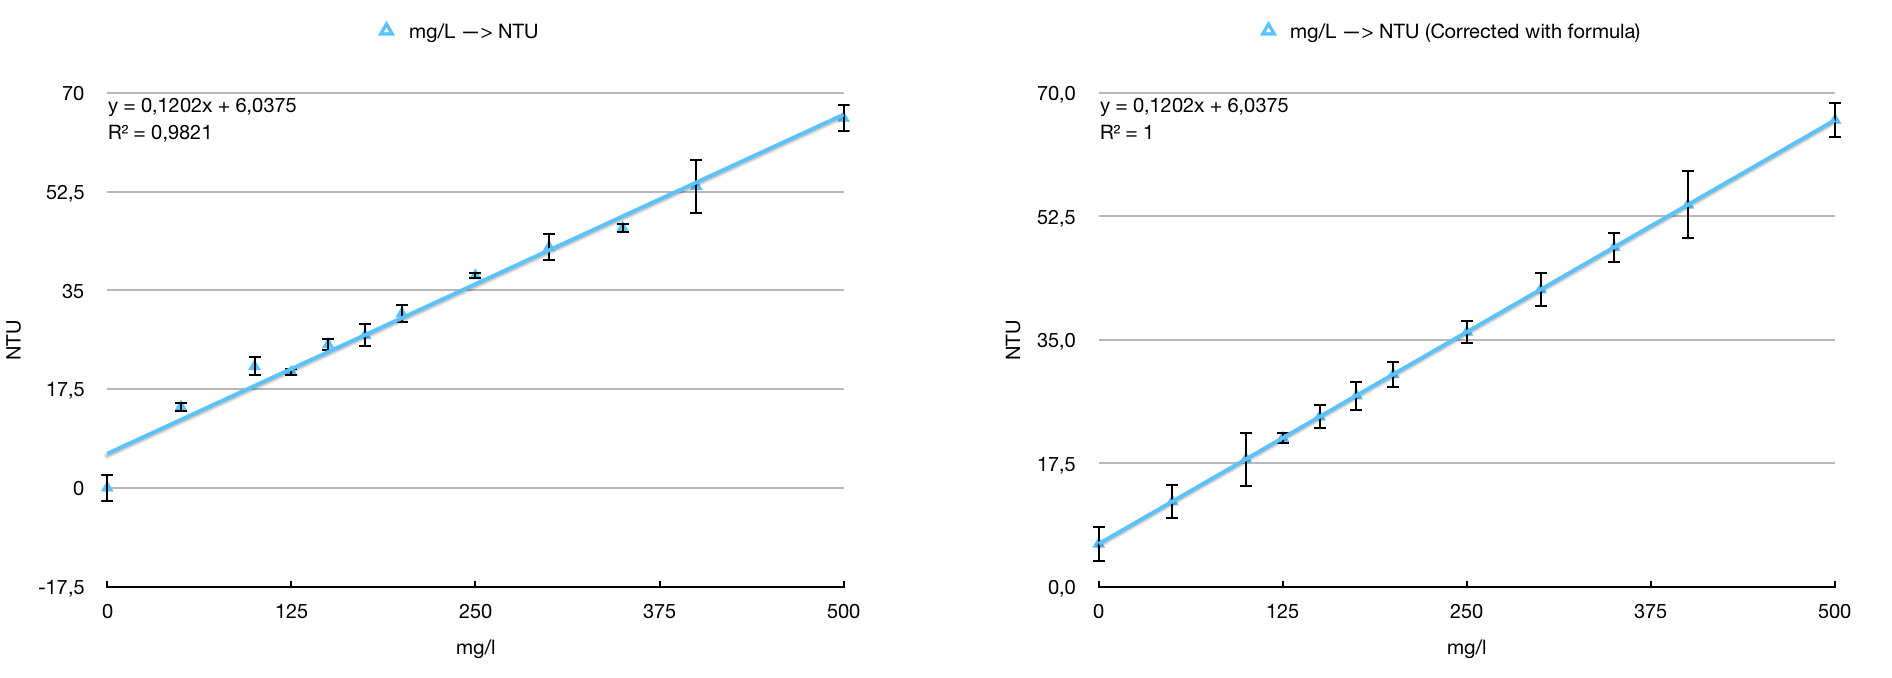
\includegraphics[width=1\linewidth]{Images/NTU_samples.png}
    \caption{Calibration of Turbidimeter AL450T-IR with measured values, trendline and standard deviation (left) and corrected values by inserting formula with standard deviation (right)}
    \label{fig:NTU_samples}
\end{figure}

\noindent The distances of the measurement points are determined by modelling the case with the round nozzle shape, as this is predicted in 3d by the model from \cite{Lee+}. In figure \ref{fig:Round_Lee} a case of the radial dispersion is shown with an outflow velocity ($u_0$) of 0.35 m/s and a height of 1.585m, like the case with the reservoir.


\begin{figure}[ht!]
    \centering
    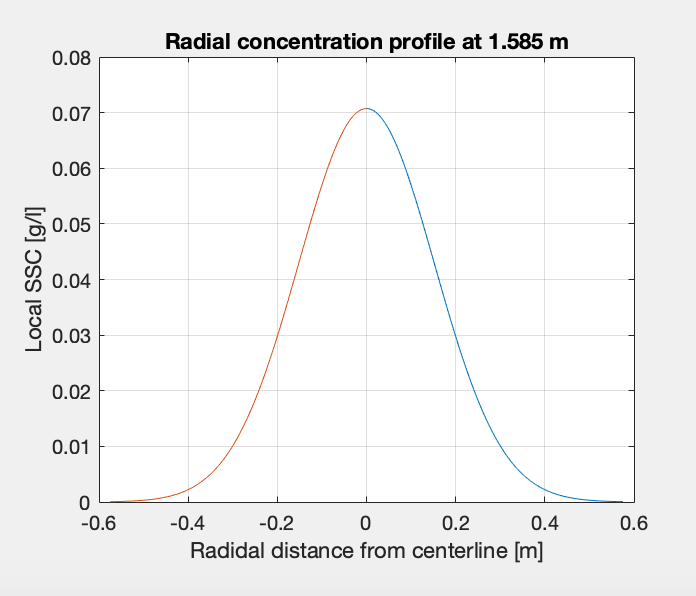
\includegraphics[width=0.3\linewidth]{Images/Round_35.png}
    \caption{Radial dispersion in case of round shape with outflow velocity ($u_0 = 0.35 m/s$), height (1.585m)}
    \label{fig:Round_Lee}
\end{figure}

\noindent Based on this model, the measurement points are decided to be in a radius from the outflow point straight down to the plate, of 100mm, 200mm, 300mm and 400mm. In table \ref{tab:measurementpoints} it is shown which measurement point is on which radius.

\begin{table}[ht!]
\centering
\begin{tabular}{|c|c|}
\hline
\textbf{Radius} & \textbf{Measurement points} \\ \hline
100 mm & 4 5 9 11 \\ \hline
200 mm & 3 9 10 12 \\ \hline
300 mm & 2 7 \\ \hline
400 mm & 1 8 \\ \hline
\end{tabular}
\caption{Overview of which measurement points lay on which radius from the middle point}
\label{tab:measurementpoints}
\end{table}


\nomenclature[Z]{NTU}{Nephelometric Turbidity Unit}

%







%plaat met meetpunten
%tab punten
%turbidimeter
\newpage
\subsection{Video imaging}
In order to get a good look whats happening during the experiments, next to the concentration measurements, two camera's are used. One camera is placed outside the tank and one GoPro camera is used inside the tank. The outside placed camera looks at the plume horizontally where the GoPro camera is placed near the outflow pipe and looks downward to visualize a top view of the plume. An overview of the placement of the camera's is shown in figure \ref{fig:camera}.

\begin{figure}[ht!]
    \centering
    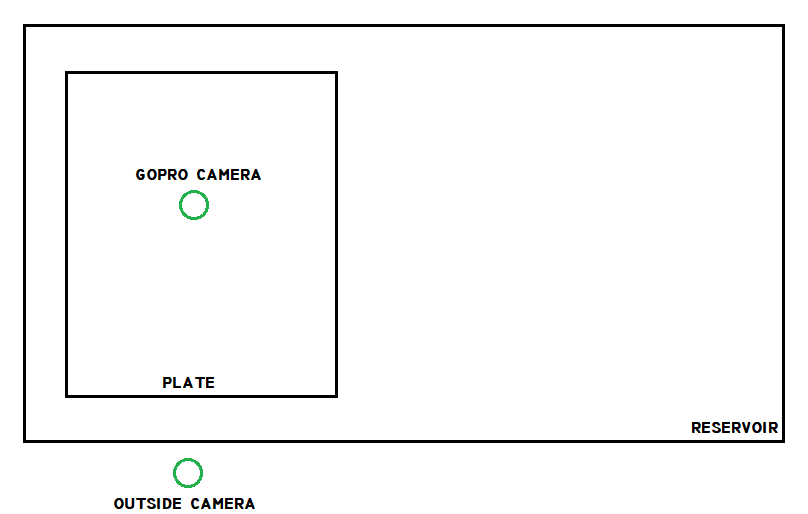
\includegraphics[width=0.6\textwidth]{Images/Camera_overzicht.png}
    \caption{Top view of placement of camera's used during experiments }
    \label{fig:camera}
\end{figure}

\nomenclature[A]{$3d$}{Three Dimensional}

%Foto contrast foto
%Foto excel bestand


\noindent As shown above, a top view and horizontal view are made by the camera's to get a good overview of the plume. The top view is used to determine the 3d shape of the plume and the camera outside shows a horizontal front view of the plume. Both camera's can say something about the differences between overflow shapes, but in other perspectives. Therefore both camera's are used to analyze the plume and to show differences between the plumes, regarding different overflow shapes. Both camera's are filming in full HD (1920x1080 pixels) and with the same framerate (25 fps). \newline
\noindent The outside camera is used to determine the angle of the plume, in 2d perspective. This is done by analyzing the movie in matlab, where the movie is edited and analyzed. The matlab script creates multiple snapshots in time with a high contrast value so that the plume is highly visible and the edges of the plume can be distinguished from the ambient water. Based on the snapshots, like figure \ref{fig:snapshot}, an overview can be made of the plume in steady state and based on this snapshot a angle is measured. 

\begin{figure}[ht!]
    \centering
    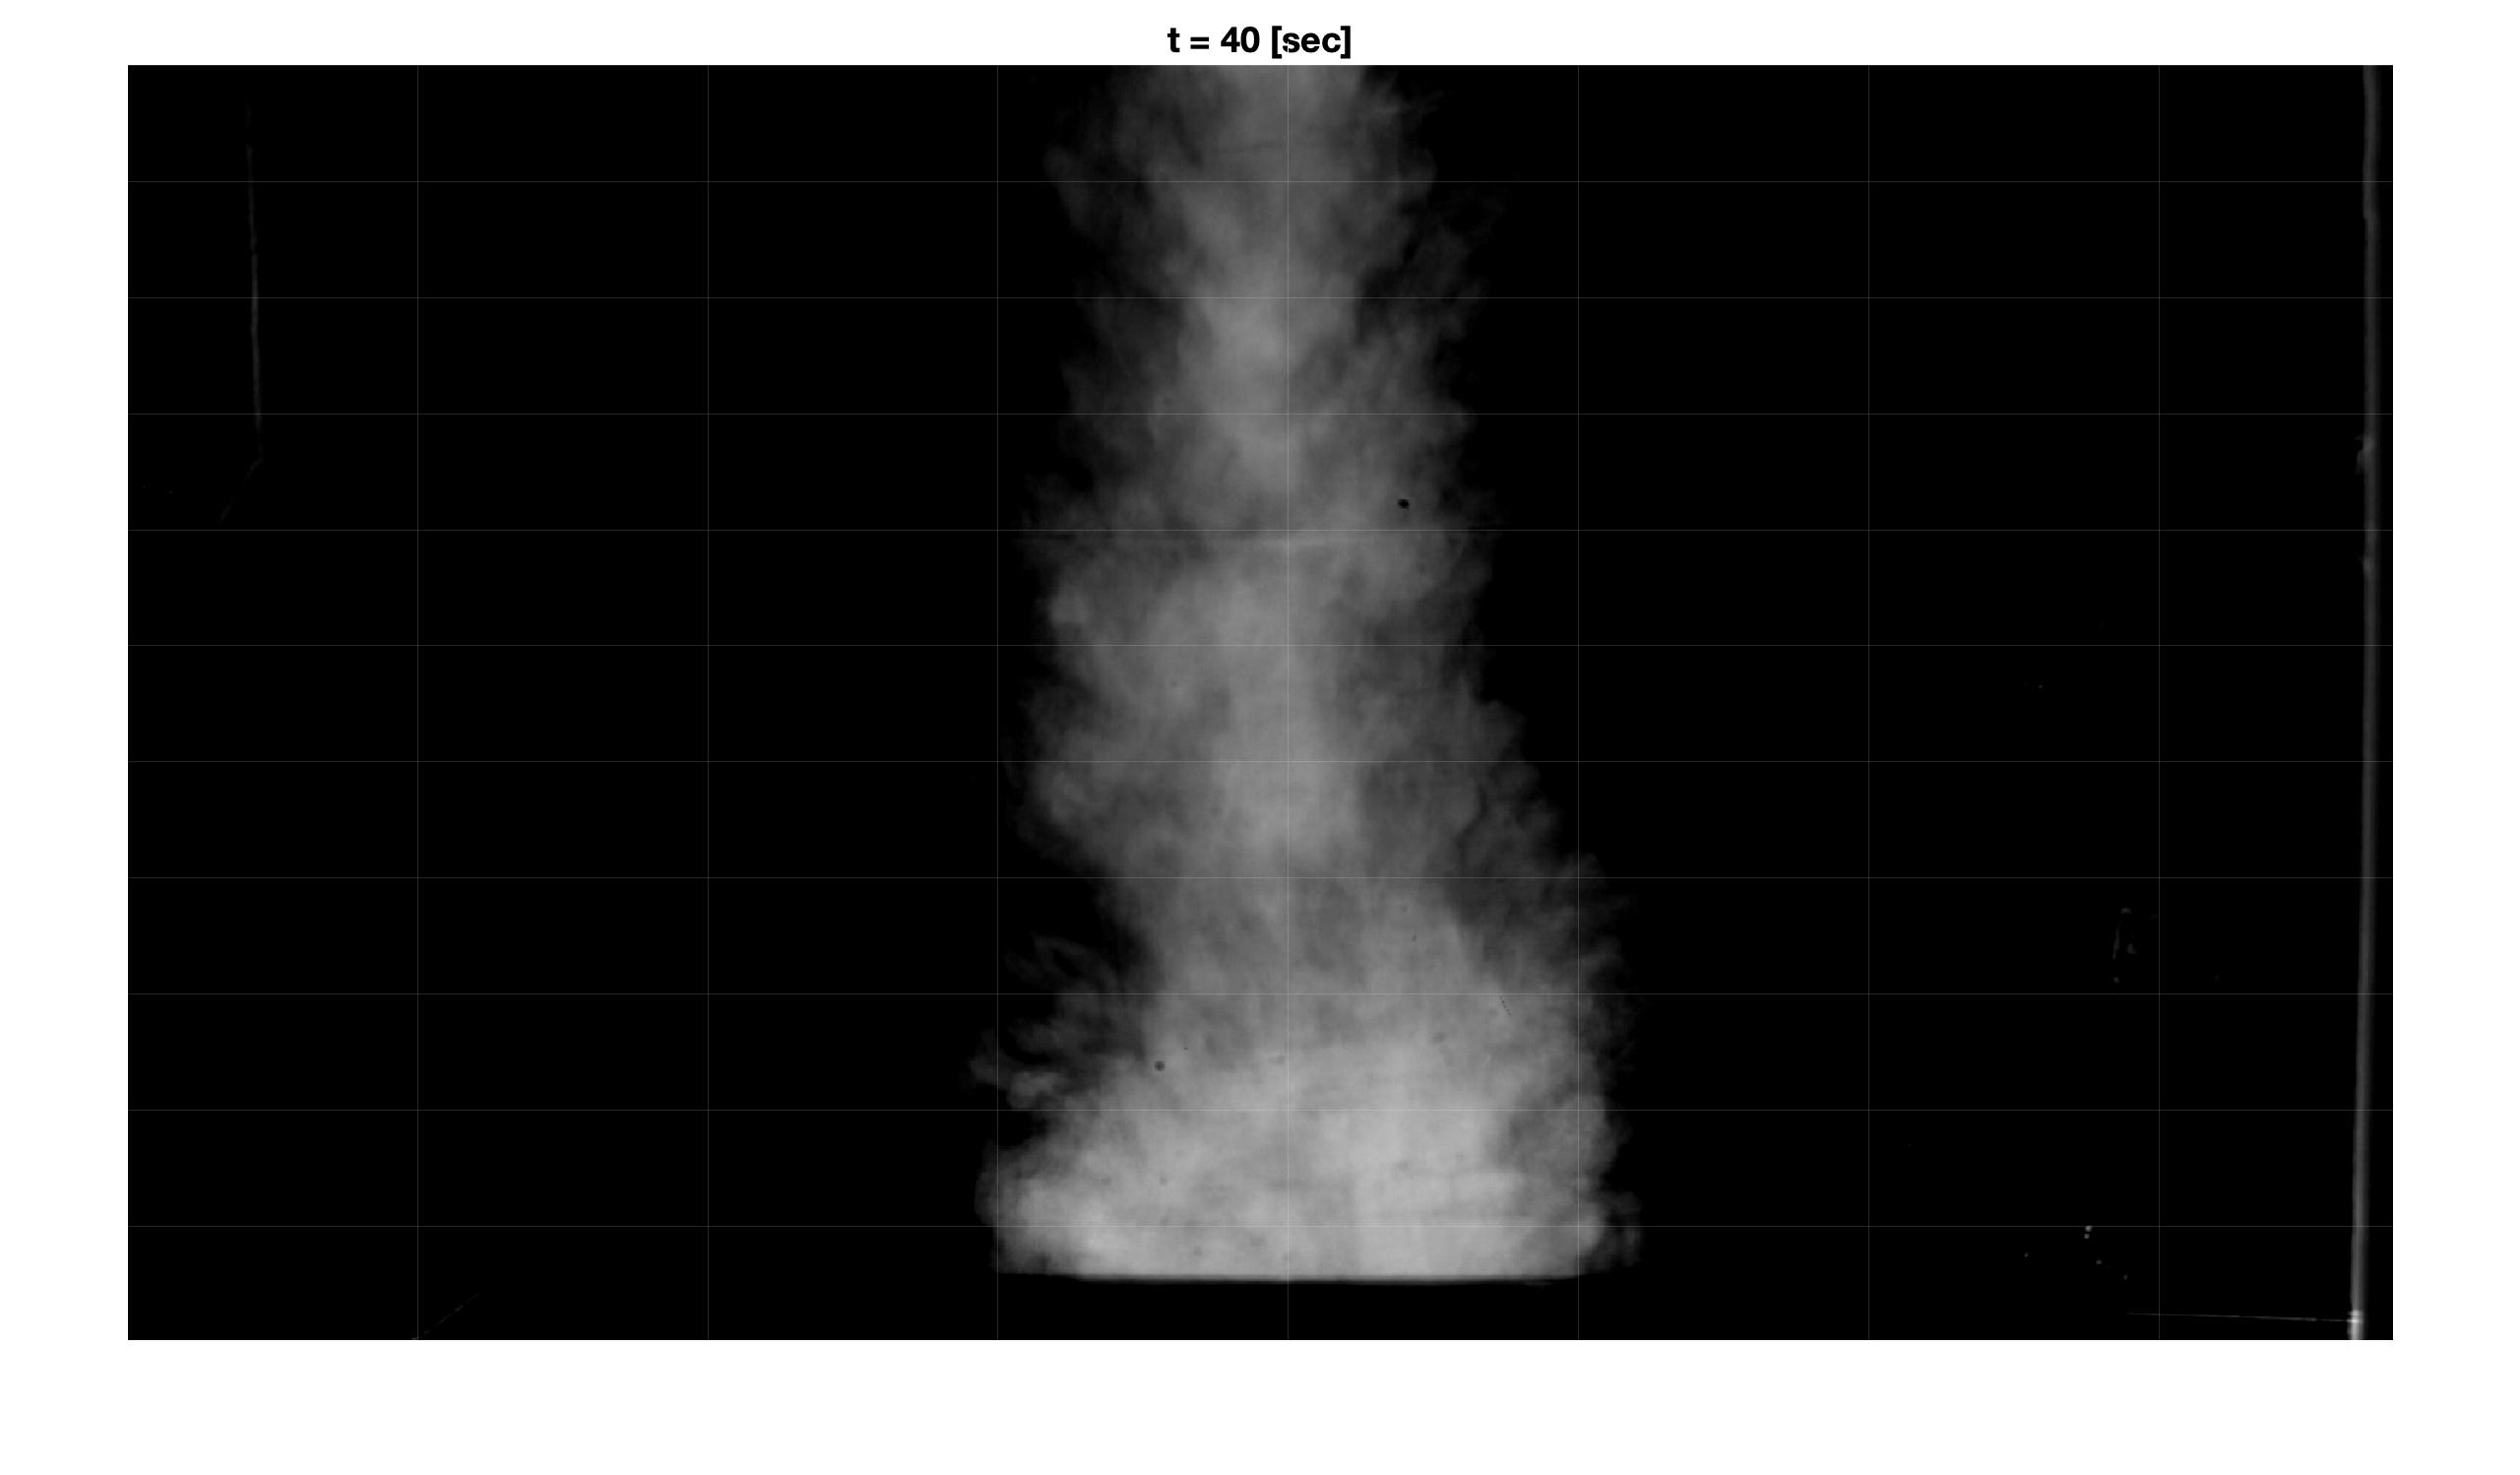
\includegraphics[width=0.6\textwidth]{Images/Round_5_t40.jpg}
    \caption{High contrast snapshot taken from camera, edited in matlab}
    \label{fig:snapshot}
\end{figure}


\begin{figure}[ht!]
    \centering
    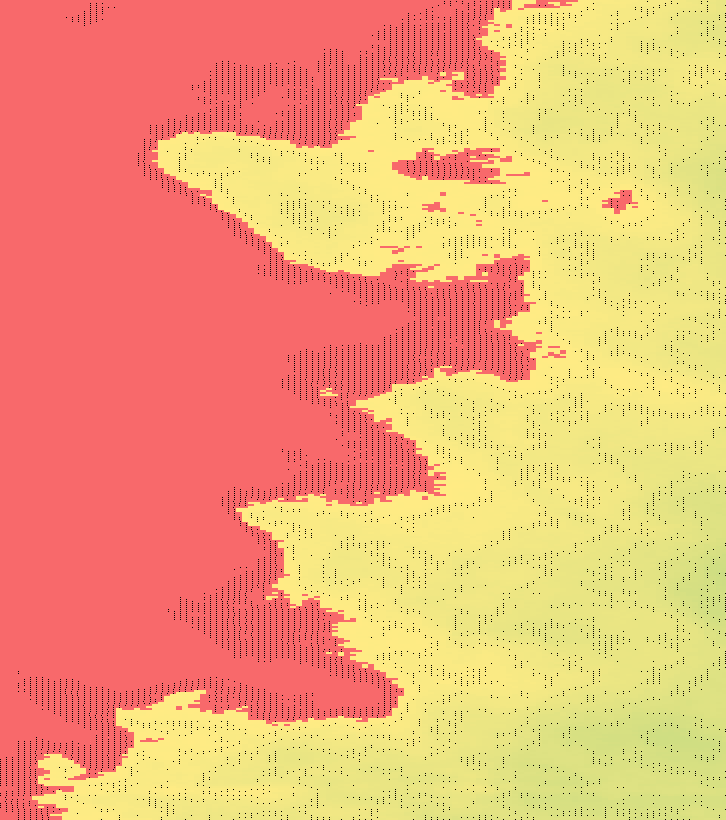
\includegraphics[width=0.4\textwidth]{Images/Colourscheme_voorbeeld.png}
    \caption{Colour scheme of plume, edited in Microsoft Excel}
    \label{fig:Excel}
\end{figure}
\newpage
\noindent The matlab script shows a matrix of 1920x1080, which are the camera pixels, with different values in them where a value of 0 is black (as shown on the snapshot) and a value of >0 is a certain white value. With this matrix, the edges of the plume are shown in numbers based on the pixels of the camera. This matrix is imported to Microsoft Excel where a colour scheme (figure \ref{fig:Excel}) is added to visualize the plume by colours. Based on this colour scheme, the edges of the plume are confirmed and a trendline is made of the left edge and the right edge of the plume. With these trendlines, the mean angle is calculated of the plume.
















\section{Experimental plan}
\label{sec:scenario}

A total of 45 experiments are done during this thesis. Test numbers 1 to 5, are concentration and angle measurements both done in one experiment. Test number 6-20 are angle measurements only for the purpose of getting a reliable angle and so entrainment coefficient. In the case of the rectangular nozzle shapes test numbers 11-20, the nozzle was turned 90 degrees to see if the angle was different. The tests where done in a multiple of 5, until a error margin of the angle was reached of $ \leq 1 ^\circ$. In table \ref{tab:ex_plan} are all parameters shown during each experiment.



%Verschil uitleggen tussen alle experimenten 1-5,6-10,11-20 etc. Testen in meervoud van 5 gedaan, stoppen indien foutmarge onder 1 graad is.



\newpage

\begin{table}
\centering
\begin{adjustbox}{max width = \linewidth}
\begin{tabular}{lcccccccc}
\hline
\multicolumn{1}{|c|}{\multirow{2}{*}{\textbf{Test \#}}} & \multicolumn{1}{c|}{\textbf{Overflow nozzle}} & \multicolumn{1}{c|}{\textbf{Inner size}} & \multicolumn{1}{c|}{\textbf{SSC}} & \multicolumn{1}{c|}{\bm{$\rho_0$}} & \multicolumn{1}{c|}{\textbf{Discharge pump}} & \multicolumn{1}{c|}{\textbf{Outflow velocity}} & \multicolumn{1}{c|}{\textbf{Discharge height}} & \multicolumn{1}{c|}{\textbf{Temperature water}} \\ \cline{2-9} 
\multicolumn{1}{|c|}{} & \multicolumn{1}{c|}{$[round / rectangular]$} & \multicolumn{1}{c|}{$[mm]$} & \multicolumn{1}{c|}{$[g/L]$} & \multicolumn{1}{c|}{$[kg / m^3]$} & \multicolumn{1}{c|}{$[l/min]$} & \multicolumn{1}{c|}{$[m/s]$} & \multicolumn{1}{c|}{$[m]$} & \multicolumn{1}{c|}{$[^\circ]$} \\ \hline
\multicolumn{1}{|l|}{Round\_1} & \multicolumn{1}{c|}{Round} & \multicolumn{1}{c|}{10} & \multicolumn{1}{c|}{5} & \multicolumn{1}{c|}{998} & \multicolumn{1}{c|}{1.641} & \multicolumn{1}{c|}{0.348} & \multicolumn{1}{c|}{1.585} & \multicolumn{1}{c|}{15.3} \\ \hline
\multicolumn{1}{|l|}{Round\_2} & \multicolumn{1}{c|}{Round} & \multicolumn{1}{c|}{10} & \multicolumn{1}{c|}{5} & \multicolumn{1}{c|}{998} & \multicolumn{1}{c|}{1.746} & \multicolumn{1}{c|}{0.371} & \multicolumn{1}{c|}{1.585} & \multicolumn{1}{c|}{15.1} \\ \hline
\multicolumn{1}{|l|}{Round\_3} & \multicolumn{1}{c|}{Round} & \multicolumn{1}{c|}{10} & \multicolumn{1}{c|}{5} & \multicolumn{1}{c|}{998} & \multicolumn{1}{c|}{1.621} & \multicolumn{1}{c|}{0.344} & \multicolumn{1}{c|}{1.585} & \multicolumn{1}{c|}{15.8} \\ \hline
\multicolumn{1}{|l|}{Round\_4} & \multicolumn{1}{c|}{Round} & \multicolumn{1}{c|}{10} & \multicolumn{1}{c|}{5} & \multicolumn{1}{c|}{998} & \multicolumn{1}{c|}{1.699} & \multicolumn{1}{c|}{0.361} & \multicolumn{1}{c|}{1.585} & \multicolumn{1}{c|}{16.3} \\ \hline
\multicolumn{1}{|l|}{Round\_5} & \multicolumn{1}{c|}{Round} & \multicolumn{1}{c|}{10} & \multicolumn{1}{c|}{5} & \multicolumn{1}{c|}{998} & \multicolumn{1}{c|}{1.644} & \multicolumn{1}{c|}{0.349} & \multicolumn{1}{c|}{1.585} & \multicolumn{1}{c|}{16.5} \\ \hline
\multicolumn{1}{|l|}{Rectangular\_20x3.9\_1} & \multicolumn{1}{c|}{Rectangular} & \multicolumn{1}{c|}{20x3.9} & \multicolumn{1}{c|}{5} & \multicolumn{1}{c|}{998} & \multicolumn{1}{c|}{1.720} & \multicolumn{1}{c|}{0.365} & \multicolumn{1}{c|}{1.585} & \multicolumn{1}{c|}{17.0} \\ \hline
\multicolumn{1}{|l|}{Rectangular\_20x3.9\_2} & \multicolumn{1}{c|}{Rectangular} & \multicolumn{1}{c|}{20x3.9} & \multicolumn{1}{c|}{5} & \multicolumn{1}{c|}{998} & \multicolumn{1}{c|}{1.661} & \multicolumn{1}{c|}{0.352} & \multicolumn{1}{c|}{1.585} & \multicolumn{1}{c|}{17.2} \\ \hline
\multicolumn{1}{|l|}{Rectangular\_20x3.9\_3} & \multicolumn{1}{c|}{Rectangular} & \multicolumn{1}{c|}{20x3.9} & \multicolumn{1}{c|}{5} & \multicolumn{1}{c|}{998} & \multicolumn{1}{c|}{1.684} & \multicolumn{1}{c|}{0.357} & \multicolumn{1}{c|}{1.585} & \multicolumn{1}{c|}{17.1} \\ \hline
\multicolumn{1}{|l|}{Rectangular\_20x3.9\_4} & \multicolumn{1}{c|}{Rectangular} & \multicolumn{1}{c|}{20x3.9} & \multicolumn{1}{c|}{5} & \multicolumn{1}{c|}{998} & \multicolumn{1}{c|}{1.583} & \multicolumn{1}{c|}{0.336} & \multicolumn{1}{c|}{1.585} & \multicolumn{1}{c|}{17.2} \\ \hline
\multicolumn{1}{|l|}{Rectangular\_20x3.9\_5} & \multicolumn{1}{c|}{Rectangular} & \multicolumn{1}{c|}{20x3.9} & \multicolumn{1}{c|}{5} & \multicolumn{1}{c|}{998} & \multicolumn{1}{c|}{1.617} & \multicolumn{1}{c|}{0.343} & \multicolumn{1}{c|}{1.585} & \multicolumn{1}{c|}{17.2} \\ \hline
\multicolumn{1}{|l|}{Rectangular\_20x3.9\_6} & \multicolumn{1}{c|}{Rectangular} & \multicolumn{1}{c|}{20x3.9} & \multicolumn{1}{c|}{5} & \multicolumn{1}{c|}{998} & \multicolumn{1}{c|}{1.593} & \multicolumn{1}{c|}{0.338} & \multicolumn{1}{c|}{1.585} & \multicolumn{1}{c|}{17.0} \\ \hline
\multicolumn{1}{|l|}{Rectangular\_20x3.9\_7} & \multicolumn{1}{c|}{Rectangular} & \multicolumn{1}{c|}{20x3.9} & \multicolumn{1}{c|}{5} & \multicolumn{1}{c|}{998} & \multicolumn{1}{c|}{1.735} & \multicolumn{1}{c|}{0.368} & \multicolumn{1}{c|}{1.585} & \multicolumn{1}{c|}{17.0} \\ \hline
\multicolumn{1}{|l|}{Rectangular\_20x3.9\_8} & \multicolumn{1}{c|}{Rectangular} & \multicolumn{1}{c|}{20x3.9} & \multicolumn{1}{c|}{5} & \multicolumn{1}{c|}{998} & \multicolumn{1}{c|}{1.601} & \multicolumn{1}{c|}{0.340} & \multicolumn{1}{c|}{1.585} & \multicolumn{1}{c|}{17.1} \\ \hline
\multicolumn{1}{|l|}{Rectangular\_20x3.9\_9} & \multicolumn{1}{c|}{Rectangular} & \multicolumn{1}{c|}{20x3.9} & \multicolumn{1}{c|}{5} & \multicolumn{1}{c|}{998} & \multicolumn{1}{c|}{1.671} & \multicolumn{1}{c|}{0.355} & \multicolumn{1}{c|}{1.585} & \multicolumn{1}{c|}{17.2} \\ \hline
\multicolumn{1}{|l|}{Rectangular\_20x3.9\_10} & \multicolumn{1}{c|}{Rectangular} & \multicolumn{1}{c|}{20x3.9} & \multicolumn{1}{c|}{5} & \multicolumn{1}{c|}{998} & \multicolumn{1}{c|}{1.678} & \multicolumn{1}{c|}{0.356} & \multicolumn{1}{c|}{1.585} & \multicolumn{1}{c|}{17.2} \\ \hline
\multicolumn{1}{|l|}{Rectangular\_20x3.9\_11} & \multicolumn{1}{c|}{Rectangular} & \multicolumn{1}{c|}{20x3.9} & \multicolumn{1}{c|}{5} & \multicolumn{1}{c|}{998} & \multicolumn{1}{c|}{1.692} & \multicolumn{1}{c|}{0.359} & \multicolumn{1}{c|}{1.585} & \multicolumn{1}{c|}{17.2} \\ \hline
\multicolumn{1}{|l|}{Rectangular\_20x3.9\_12} & \multicolumn{1}{c|}{Rectangular} & \multicolumn{1}{c|}{20x3.9} & \multicolumn{1}{c|}{5} & \multicolumn{1}{c|}{998} & \multicolumn{1}{c|}{1.662} & \multicolumn{1}{c|}{0.353} & \multicolumn{1}{c|}{1.585} & \multicolumn{1}{c|}{17.2} \\ \hline
\multicolumn{1}{|l|}{Rectangular\_20x3.9\_13} & \multicolumn{1}{c|}{Rectangular} & \multicolumn{1}{c|}{20x3.9} & \multicolumn{1}{c|}{5} & \multicolumn{1}{c|}{998} & \multicolumn{1}{c|}{1.664} & \multicolumn{1}{c|}{0.353} & \multicolumn{1}{c|}{1.585} & \multicolumn{1}{c|}{17.2} \\ \hline
\multicolumn{1}{|l|}{Rectangular\_20x3.9\_14} & \multicolumn{1}{c|}{Rectangular} & \multicolumn{1}{c|}{20x3.9} & \multicolumn{1}{c|}{5} & \multicolumn{1}{c|}{998} & \multicolumn{1}{c|}{1.623} & \multicolumn{1}{c|}{0.344} & \multicolumn{1}{c|}{1.585} & \multicolumn{1}{c|}{17.2} \\ \hline
\multicolumn{1}{|l|}{Rectangular\_20x3.9\_15} & \multicolumn{1}{c|}{Rectangular} & \multicolumn{1}{c|}{20x3.9} & \multicolumn{1}{c|}{5} & \multicolumn{1}{c|}{998} & \multicolumn{1}{c|}{1.704} & \multicolumn{1}{c|}{0.362} & \multicolumn{1}{c|}{1.585} & \multicolumn{1}{c|}{17.2} \\ \hline
\multicolumn{1}{|l|}{Rectangular\_20x3.9\_16} & \multicolumn{1}{c|}{Rectangular} & \multicolumn{1}{c|}{20x3.9} & \multicolumn{1}{c|}{5} & \multicolumn{1}{c|}{998} & \multicolumn{1}{c|}{1.575} & \multicolumn{1}{c|}{0.334} & \multicolumn{1}{c|}{1.585} & \multicolumn{1}{c|}{17.2} \\ \hline
\multicolumn{1}{|l|}{Rectangular\_20x3.9\_17} & \multicolumn{1}{c|}{Rectangular} & \multicolumn{1}{c|}{20x3.9} & \multicolumn{1}{c|}{5} & \multicolumn{1}{c|}{998} & \multicolumn{1}{c|}{1.753} & \multicolumn{1}{c|}{0.372} & \multicolumn{1}{c|}{1.585} & \multicolumn{1}{c|}{17.2} \\ \hline
\multicolumn{1}{|l|}{Rectangular\_20x3.9\_18} & \multicolumn{1}{c|}{Rectangular} & \multicolumn{1}{c|}{20x3.9} & \multicolumn{1}{c|}{5} & \multicolumn{1}{c|}{998} & \multicolumn{1}{c|}{1.596} & \multicolumn{1}{c|}{0.339} & \multicolumn{1}{c|}{1.585} & \multicolumn{1}{c|}{17.2} \\ \hline
\multicolumn{1}{|l|}{Rectangular\_20x3.9\_19} & \multicolumn{1}{c|}{Rectangular} & \multicolumn{1}{c|}{20x3.9} & \multicolumn{1}{c|}{5} & \multicolumn{1}{c|}{998} & \multicolumn{1}{c|}{1.672} & \multicolumn{1}{c|}{0.355} & \multicolumn{1}{c|}{1.585} & \multicolumn{1}{c|}{17.5} \\ \hline
\multicolumn{1}{|l|}{Rectangular\_20x3.9\_20} & \multicolumn{1}{c|}{Rectangular} & \multicolumn{1}{c|}{20x3.9} & \multicolumn{1}{c|}{5} & \multicolumn{1}{c|}{998} & \multicolumn{1}{c|}{1.673} & \multicolumn{1}{c|}{0.355} & \multicolumn{1}{c|}{1.585} & \multicolumn{1}{c|}{17.5} \\ \hline
\multicolumn{1}{|l|}{Rectangular\_30x2.6\_1} & \multicolumn{1}{c|}{Rectangular} & \multicolumn{1}{c|}{30x2.6} & \multicolumn{1}{c|}{5} & \multicolumn{1}{c|}{998} & \multicolumn{1}{c|}{1.593} & \multicolumn{1}{c|}{0.338} & \multicolumn{1}{c|}{1.585} & \multicolumn{1}{c|}{17.7} \\ \hline
\multicolumn{1}{|l|}{Rectangular\_30x2.6\_2} & \multicolumn{1}{c|}{Rectangular} & \multicolumn{1}{c|}{30x2.6} & \multicolumn{1}{c|}{5} & \multicolumn{1}{c|}{998} & \multicolumn{1}{c|}{1.653} & \multicolumn{1}{c|}{0.351} & \multicolumn{1}{c|}{1.585} & \multicolumn{1}{c|}{17.9} \\ \hline
\multicolumn{1}{|l|}{Rectangular\_30x2.6\_3} & \multicolumn{1}{c|}{Rectangular} & \multicolumn{1}{c|}{30x2.6} & \multicolumn{1}{c|}{5} & \multicolumn{1}{c|}{998} & \multicolumn{1}{c|}{1.618} & \multicolumn{1}{c|}{0.343} & \multicolumn{1}{c|}{1.585} & \multicolumn{1}{c|}{17.9} \\ \hline
\multicolumn{1}{|l|}{Rectangular\_30x2.6\_4} & \multicolumn{1}{c|}{Rectangular} & \multicolumn{1}{c|}{30x2.6} & \multicolumn{1}{c|}{5} & \multicolumn{1}{c|}{998} & \multicolumn{1}{c|}{1.596} & \multicolumn{1}{c|}{0.339} & \multicolumn{1}{c|}{1.585} & \multicolumn{1}{c|}{17.9} \\ \hline
\multicolumn{1}{|l|}{Rectangular\_30x2.6\_5} & \multicolumn{1}{c|}{Rectangular} & \multicolumn{1}{c|}{30x2.6} & \multicolumn{1}{c|}{5} & \multicolumn{1}{c|}{998} & \multicolumn{1}{c|}{1.540} & \multicolumn{1}{c|}{0.327} & \multicolumn{1}{c|}{1.585} & \multicolumn{1}{c|}{17.9} \\ \hline
\multicolumn{1}{|l|}{Rectangular\_30x2.6\_6} & \multicolumn{1}{c|}{Rectangular} & \multicolumn{1}{c|}{30x2.6} & \multicolumn{1}{c|}{5} & \multicolumn{1}{c|}{998} & \multicolumn{1}{c|}{1.655} & \multicolumn{1}{c|}{0.351} & \multicolumn{1}{c|}{1.585} & \multicolumn{1}{c|}{17.9} \\ \hline
\multicolumn{1}{|l|}{Rectangular\_30x2.6\_7} & \multicolumn{1}{c|}{Rectangular} & \multicolumn{1}{c|}{30x2.6} & \multicolumn{1}{c|}{5} & \multicolumn{1}{c|}{998} & \multicolumn{1}{c|}{1.653} & \multicolumn{1}{c|}{0.351} & \multicolumn{1}{c|}{1.585} & \multicolumn{1}{c|}{17.9} \\ \hline
\multicolumn{1}{|l|}{Rectangular\_30x2.6\_8} & \multicolumn{1}{c|}{Rectangular} & \multicolumn{1}{c|}{30x2.6} & \multicolumn{1}{c|}{5} & \multicolumn{1}{c|}{998} & \multicolumn{1}{c|}{1.644} & \multicolumn{1}{c|}{0.349} & \multicolumn{1}{c|}{1.585} & \multicolumn{1}{c|}{17.9} \\ \hline
\multicolumn{1}{|l|}{Rectangular\_30x2.6\_9} & \multicolumn{1}{c|}{Rectangular} & \multicolumn{1}{c|}{30x2.6} & \multicolumn{1}{c|}{5} & \multicolumn{1}{c|}{998} & \multicolumn{1}{c|}{1.623} & \multicolumn{1}{c|}{0.344} & \multicolumn{1}{c|}{1.585} & \multicolumn{1}{c|}{17.9} \\ \hline
\multicolumn{1}{|l|}{Rectangular\_30x2.6\_10} & \multicolumn{1}{c|}{Rectangular} & \multicolumn{1}{c|}{30x2.6} & \multicolumn{1}{c|}{5} & \multicolumn{1}{c|}{998} & \multicolumn{1}{c|}{1.654} & \multicolumn{1}{c|}{0.351} & \multicolumn{1}{c|}{1.585} & \multicolumn{1}{c|}{17.9} \\ \hline
\multicolumn{1}{|l|}{Rectangular\_30x2.6\_11} & \multicolumn{1}{c|}{Rectangular} & \multicolumn{1}{c|}{30x2.6} & \multicolumn{1}{c|}{5} & \multicolumn{1}{c|}{998} & \multicolumn{1}{c|}{1.713} & \multicolumn{1}{c|}{0.364} & \multicolumn{1}{c|}{1.585} & \multicolumn{1}{c|}{17.9} \\ \hline
\multicolumn{1}{|l|}{Rectangular\_30x2.6\_12} & \multicolumn{1}{c|}{Rectangular} & \multicolumn{1}{c|}{30x2.6} & \multicolumn{1}{c|}{5} & \multicolumn{1}{c|}{998} & \multicolumn{1}{c|}{1.649} & \multicolumn{1}{c|}{0.350} & \multicolumn{1}{c|}{1.585} & \multicolumn{1}{c|}{17.9} \\ \hline
\multicolumn{1}{|l|}{Rectangular\_30x2.6\_13} & \multicolumn{1}{c|}{Rectangular} & \multicolumn{1}{c|}{30x2.6} & \multicolumn{1}{c|}{5} & \multicolumn{1}{c|}{998} & \multicolumn{1}{c|}{1.679} & \multicolumn{1}{c|}{0.356} & \multicolumn{1}{c|}{1.585} & \multicolumn{1}{c|}{17.9} \\ \hline
\multicolumn{1}{|l|}{Rectangular\_30x2.6\_14} & \multicolumn{1}{c|}{Rectangular} & \multicolumn{1}{c|}{30x2.6} & \multicolumn{1}{c|}{5} & \multicolumn{1}{c|}{998} & \multicolumn{1}{c|}{1.709} & \multicolumn{1}{c|}{0.363} & \multicolumn{1}{c|}{1.585} & \multicolumn{1}{c|}{17.9} \\ \hline
\multicolumn{1}{|l|}{Rectangular\_30x2.6\_15} & \multicolumn{1}{c|}{Rectangular} & \multicolumn{1}{c|}{30x2.6} & \multicolumn{1}{c|}{5} & \multicolumn{1}{c|}{998} & \multicolumn{1}{c|}{1.661} & \multicolumn{1}{c|}{0.352} & \multicolumn{1}{c|}{1.585} & \multicolumn{1}{c|}{17.9} \\ \hline
\multicolumn{1}{|l|}{Rectangular\_30x2.6\_16} & \multicolumn{1}{c|}{Rectangular} & \multicolumn{1}{c|}{30x2.6} & \multicolumn{1}{c|}{5} & \multicolumn{1}{c|}{998} & \multicolumn{1}{c|}{1.688} & \multicolumn{1}{c|}{0.358} & \multicolumn{1}{c|}{1.585} & \multicolumn{1}{c|}{17.9} \\ \hline
\multicolumn{1}{|l|}{Rectangular\_30x2.6\_17} & \multicolumn{1}{c|}{Rectangular} & \multicolumn{1}{c|}{30x2.6} & \multicolumn{1}{c|}{5} & \multicolumn{1}{c|}{998} & \multicolumn{1}{c|}{1.670} & \multicolumn{1}{c|}{0.354} & \multicolumn{1}{c|}{1.585} & \multicolumn{1}{c|}{17.9} \\ \hline
\multicolumn{1}{|l|}{Rectangular\_30x2.6\_18} & \multicolumn{1}{c|}{Rectangular} & \multicolumn{1}{c|}{30x2.6} & \multicolumn{1}{c|}{5} & \multicolumn{1}{c|}{998} & \multicolumn{1}{c|}{1.603} & \multicolumn{1}{c|}{0.340} & \multicolumn{1}{c|}{1.585} & \multicolumn{1}{c|}{17.9} \\ \hline
\multicolumn{1}{|l|}{Rectangular\_30x2.6\_19} & \multicolumn{1}{c|}{Rectangular} & \multicolumn{1}{c|}{30x2.6} & \multicolumn{1}{c|}{5} & \multicolumn{1}{c|}{998} & \multicolumn{1}{c|}{1.627} & \multicolumn{1}{c|}{0.345} & \multicolumn{1}{c|}{1.585} & \multicolumn{1}{c|}{17.9} \\ \hline
\multicolumn{1}{|l|}{Rectangular\_30x2.6\_20} & \multicolumn{1}{c|}{Rectangular} & \multicolumn{1}{c|}{30x2.6} & \multicolumn{1}{c|}{5} & \multicolumn{1}{c|}{998} & \multicolumn{1}{c|}{1.658} & \multicolumn{1}{c|}{0.352} & \multicolumn{1}{c|}{1.585} & \multicolumn{1}{c|}{17.9} \\ \hline
 & \multicolumn{1}{l}{} & \multicolumn{1}{l}{} & \multicolumn{1}{l}{} & \multicolumn{1}{l}{} & \multicolumn{1}{l}{} & \multicolumn{1}{l}{} & \multicolumn{1}{l}{} & \multicolumn{1}{l}{}

\end{tabular}
\end{adjustbox}
\caption{Used parameters for each experiment}
\label{tab:ex_plan}
\end{table}









%Testplan zoals Georges zei ; density, materiaal, tijd blabla
%foto meetpunten plaat

%Mixture density bepalen, restrictie aan pomp/aansluiting
%Snelheid bepalen
%Concentratie meten

%Eerst vormen testen met zelfde oppervlak
%Preciese uitleg concentratiemeters 


















%\section{Previous used test methods}
%In order to come to a sufficient test setup, previous used methods are further elaborated in this section. Information from previous tests can be used in order to create a usable test setup to test an air filter and shape mold designs for the outflow of the overflow. Firstly a separation is made in past air tests and shape tests. \newline

%\noindent \textbf{Previous air test methods} \newline
%As explained in section \ref{sec:air}, \cite{Zhang+} preformed experimental tests where air and water are both injected in a current. Existing studies on either air or air–water injection in large setups were conducted mostly in stagnant ambient water and very limited in cross flow. However, cross flow is typically present in many applications, for instance dredging. Therefore \cite{Zhang+} created an experimental setup, which is shown in figure \ref{fig:Zhang_experiment}, to test the air-water injection in a cross flow. The increase of injected air showed an increase in suspended injected water, which is visible with dye (figure \ref{fig:Zhang_experiment_2}). This test concluded that air will increase the separation height with increasing air momentum. However, it cannot be used to test an air filter because air is injected and not added due to a pulsing inflow for example. \newline

%\noindent Both \cite{Dewit} and \cite{Decrop} implemented air in their models. In addition, both models were compared with an experimental setup. In both models, the relation of \cite{Ervine} is used, which estimated the amount of entrained air in an overflow without green valve as shown below.

%\begin{equation}
%\label{eq:air}
 %   q_{air} = 0.00002(w_i-1)^3 + 0.0003(w_i-1)^2 + 0.0074(w_i-1) - 0.0058
%\end{equation}


%\noindent With $q_{air}$ as the volume flux of air per metre plunging width in [$m^2/s$] and $w_i$ as the vertical impact velocity in [m/s] of a dropping water jet when it touches the water surface, 1 m/s is subtracted because minimal 1 m/s is needed for any form of aeration. $w_i$ can be related to the drop height of a water jet by the assumption of initial zero vertical velocity and constant acceleration by gravity ($\sqrt{2gH_d}$). In figure \ref{fig:aireq_dewit} the air flux $Q_{air}$ = $q_{air} \pi D$ as a function of the drop height is compared to the water flux $Q_{water}$ = $\pi/4 D^2 W_0$ in the overflow. Figure \ref{fig:aireq_dewit} shows that the percentage of entrained air depends strongly on drop height and $W_0$: between 0 and 30\% air entrainment can be expected for realistic overflow diameters in combination with realistic overflow velocities. \newline


%\nomenclature[A]{$q_{air}$}{Volume flux of air per metre plunging width \nomunit{$[m^2/s]$}}
%\nomenclature[A]{$w_i$}{Vertical impact velocity op dropping water jet on water surface touch\nomunit{$[m/s]$}}
%\nomenclature[G]{$\rho_{cf}$}{Ambient density cross flow \nomunit{$[kg/m^3]$}}


%\noindent \cite{Dewit} compared his model with experiments done by \cite{Liu}, for his MSc graduation, at the large dredging flume of Deltares. In this experiment, the dredging plume is created by injecting a saline water solution from the keel of a moving TSHD in stagnant water of $\rho_cf$ = 1000 $kg/m^3$, see figure 5.2. 



%\begin{figure}[ht!]
%    \centering
%    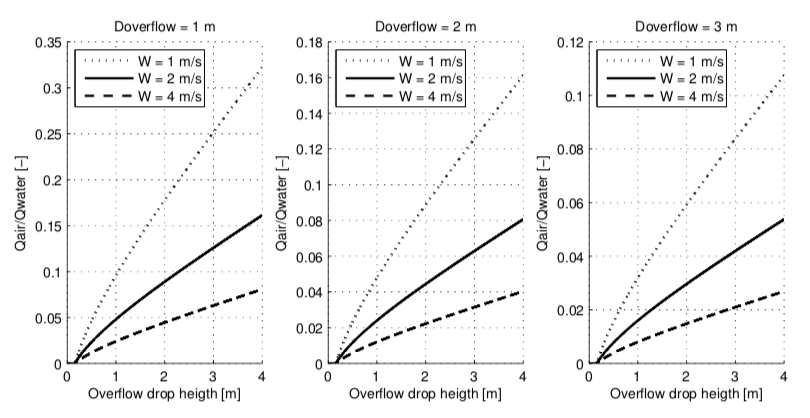
\includegraphics[width=1\textwidth]{Images/Air_dewit_2.png}
%    \caption{Estimate of the amount of entrained air in the overflow calculated with equation 5.1 as a function of the overflow drop height}
%    \label{fig:aireq_dewit}
%\end{figure}

%\begin{figure}[ht!]
%\centering
%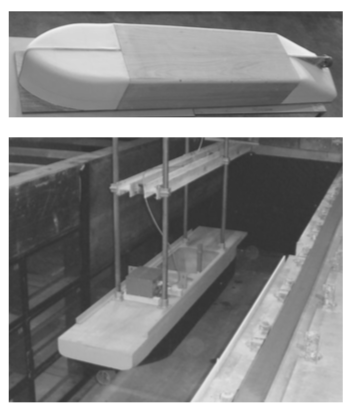
\includegraphics[width=5.5cm]{Images/experiment_dewit.png}
%\caption{Experimental setup in the large dredging flume at Deltares}
%\end{figure}

%\newpage
%\noindent \cite{Decrop} did his experiments at a 15m long flume at the Hydraulics Laboratory of Ghent University. The flume was used to host the scaled overflow plume experiments (figure \ref{fig:overview_decrop_experiment}). The flume had a width of 0.8m and a flow depth of about 0.6m was used in all cases. The mean flow velocity $U_0$ was varied between 0.1 \& 0.3 m/s. Profiles of the streamwise velocity component in the flume were verified using ADV measurements of lateral and vertical profiles. It was found that the lateral velocity profile in the flume was fairly uniform at more than 0.18m from the flume walls. The flume side walls consist of smooth panels, but the joints between the panels are most likely the cause of the wider boundary layer velocity profile, as for rough walls. The vertical profile of the streamwise velocity exhibits a logarithmic profile. At 0.1m from the bottom wall, the streamwise velocity amounted to 90\% of the maximum velocity.\newline

%\begin{figure}[ht!]
%    \centering
%    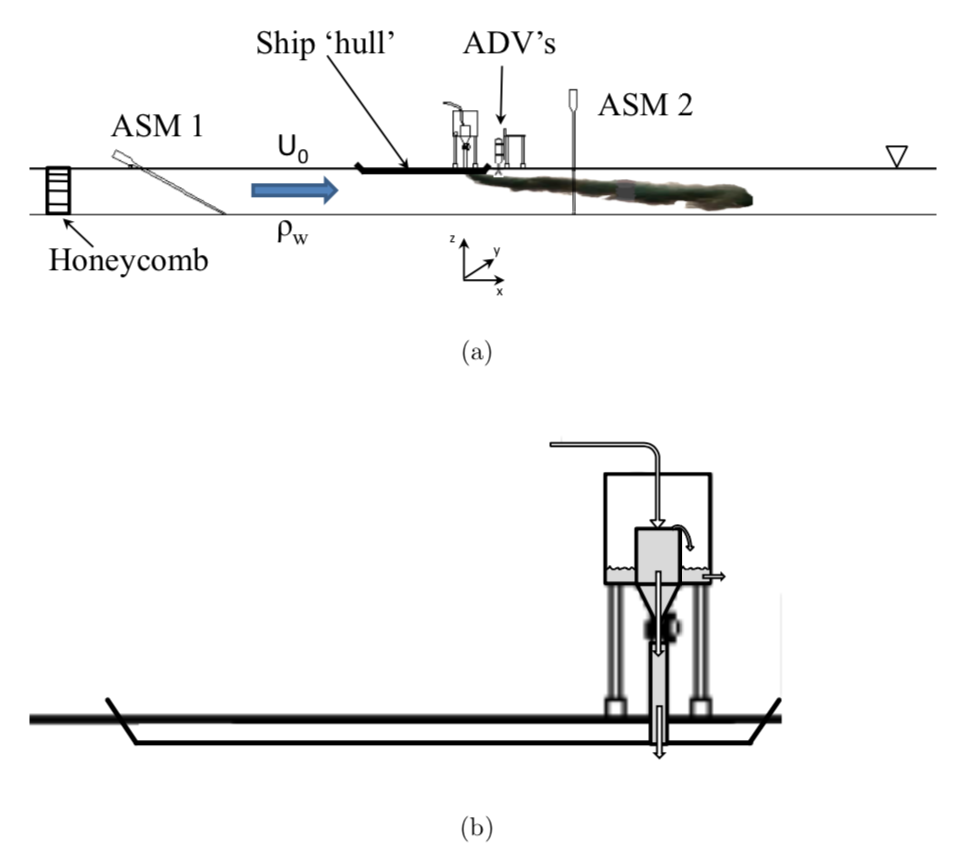
\includegraphics[width=0.8\textwidth]{Images/overview_decrop_experiment.png}
%    \caption{Top panel: Experimental setup, with a plume feeding mechanism containing a constant head vessel mounted on top of the flume. ADV and two ASM instruments installed at respectively 0.5m and 1.4m from the plume exit. Lower panel: Detail of the schematized hull and constant head vessel}
%    \label{fig:overview_decrop_experiment}
%\end{figure}



%\noindent The above observations lead to the conclusion that the studied plumes may preferably not extend further than 0.2m from the sidewalls and 0.1m from the bottom wall before reaching the measurement sections.
%\newpage
%\noindent The dredging plume experiments require the influence of a dredging vessel hull, with bow and stern section. Since the flume is too narrow to include a three-dimensional vessel hull shape without significant influence of the flume wall proximity, a schematized, two-dimensional hull was designed. To this end, a 2.12 x 0.8m poly carbonate plate was given a bow and stern section by folding the plate at 60$^{\circ}$ angles at both ends. The schematized hull is therefore laterally uniform and represents an infinitely wide vessel, in comparison to the overflow shaft pipe diameter. The overflow pipe was fitted flush with the schematized hull at a streamwise distance of 1.8 m downstream of the bow. Its axis was positioned in the direction normal to the hull plate. The stern section of the schematized hull is located at 0.32m downstream of the overflow pipe.\newline

%\noindent \cite{Decrop} used commercially available kaolin (China clay) for the fine sediment experiments for (i) its relatively low cation exchange capacity and (ii) its narrow grain size distribution. The first aspect eases the production of homogeneous mixtures, while the latter facilitates interpretation of the acoustic response, although that primary kaolin particles form micro-flocs due to their electrical charge. A second mineral was considered for execution of the plume experiments: quartz powder (ground sand M300, produced by Sibelco Benelux) was considered in the experiments for its absence of electrical charges responsible for flocculation and its particle size distribution being comparable to clays. The quartz powder was not chosen for the main plume experiment, notwithstanding its inert property due to which it does not flocculate. The particle size distribution showed some fraction of larger particles, of d >60 $\mu$m. This fraction tends to settle in the different vessels used for mixing and transporting the water-sediment mixture, reducing the control over the particle size distribution reaching the plume. 
%\newpage
%\noindent To ensure a steady plume of which the statistics stabilize over time, the water-clay mixture for the plume release is required to stay homogeneous during the course of an experiment of \cite{Decrop}. This was achieved by using a mixing vessel (figure \ref{fig:decrop_mixingtank}).
%The 0.3$m^3$ cylindrical mixing vessel has been designed for being capable of keeping a mixture of fine sediments in suspension, while providing sufficient free space for instruments to be installed and containing sufficient water-sediment mixture for a 20-minute plume experiment. A 7,500 l/h submersible pump was installed for this purpose near the bottom of the vessel. This pump is positioned with its nozzle in the centre and blows towards the bottom from a height of 0.1m, generating the required circulation at a total shear stress of about 2.5Pa (as measured by the ADV) in the centre of the vessel.

%\begin{figure}[ht!]
 %   \centering
 %   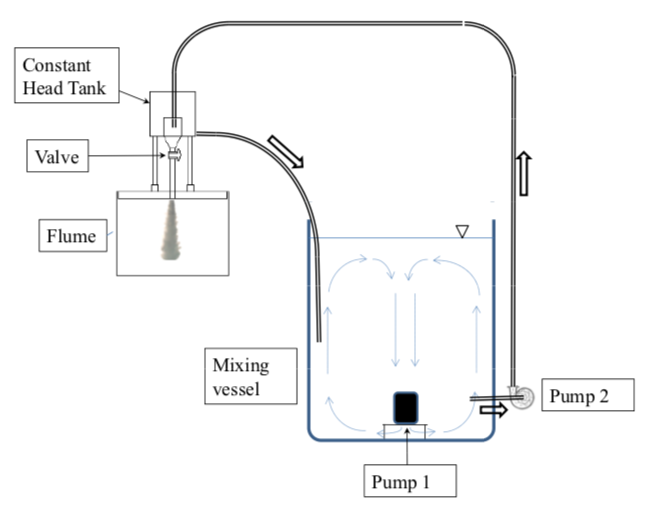
\includegraphics[width=0.5\textwidth]{Images/decrop_mixingtank.png}
 %   \caption{Plume feeding mechanism including a mixing tank, pumps and constant head vessel}
 %   \label{fig:decrop_mixingtank}
%\end{figure}


%\noindent In the specific tests of \cite{Decrop} where the influence of air bubbles is assessed, air bubbles are injected in the overflow pipe with an injection needle connected to a compressor. The injection occurs at a pressure of 3 bar and produces bubbles of various diameters in the overflow pipe. Controlling the size of air bubbles is difficult. However, only air bubbles having a rise velocity smaller than the flow velocity in the exit pipe will be released. During the air bubble experiments described in this thesis, the exit velocity was 0.3 m/s. Air bubbles in a water-sediment mixture of density equal to 1020 kg/m3 have a terminal rise velocity of 0.3 m/s at a diameter of about 3mm according to \cite{Talaia}. Only bubbles with diameter of 3mm or smaller will travel down the overflow pipe, larger bubbles rise in the constant head vessel before entering the overflow pipe. This fixes the upper limit of air bubble rise velocity to scale with the maximum air bubble rise velocity in reality. Unfortunately, the lower end of the bubble rise velocity distribution is unknown in real dredging conditions and difficult to control in an experiment. Images were taken of the air bubbles released from the overflow pipe (figure \ref{fig:decrop_air}) without sediment in the pipe flow. In a single image, no information is available about the distance of the air bubble from the camera. However, the distance from the camera to the center of the pipe is 0.4m and the width of the area containing air bubbles is about the same as the pipe diameter at short distance from the pipe. Therefore, the uncertainty on the air bubble diameter measured in this way is about 10\%. Using the pipe diameter as a ruler, the air bubble diameter is estimated to range from 0.5mm to 3mm. A small number of larger bubbles are present due to coalescence of primary bubbles. \newline

%\begin{figure}[ht!]
 %   \centering
 %   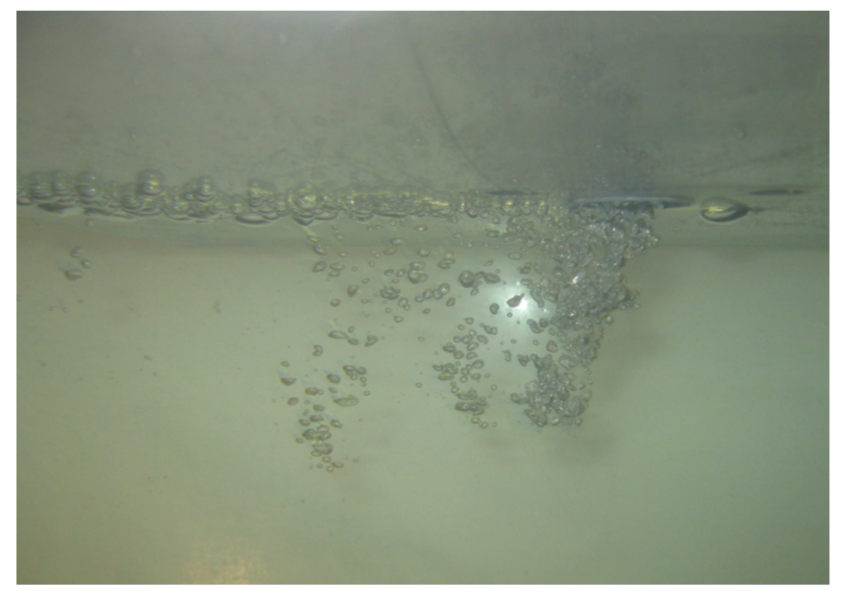
\includegraphics[width=0.5\textwidth]{Images/decrop_air.png}
 %   \caption{Image of air bubbles released from the overflow exit pipe in a plume without sediment at the same exit flow velocity as in the sediment plume experiments.}
 %   \label{fig:decrop_air}
%\end{figure}


%\noindent Further, the volume concentration of the air bubbles is determined as follows. The volume discharge released from the calibrated constant head vessel is known. First, the volume discharge of water-sediment mixture $Q_0$ is measured by timing the release of a given volume of mixture from the reservoir, of which the result has to be in accordance with the constant head vessel calibration. Then the air bubble release mechanism is turned on, after which the same measurement is taken, resulting in the volume discharge of the mixture in the presence of air bubbles $Q_{m,a}$. The air bubble volume concentration or void fraction $\theta_a$ is determined from equation \ref{eq:Q}.
%\begin{equation}
 %   Q_a =\theta_a Q_0 = Q_0 - Q_{m,a} 
 %   \label{eq:Q}
%\end{equation}

%\nomenclature[A]{$Q_a$}{}



%\newpage
%\noindent The void fraction obtained in the experiments by \cite{Decrop} was between 9\% and 30\%. Shortly after release, the larger air bubbles rise to the bottom of the polycarbonate plate representing the TSHD hull, whereas the smaller bubbles are ejected further from the exit and are entrained with the mean flow. However, since the rise velocity of the bubbles is of the same order of magnitude as the horizontal mean flow the bubbles reach the hull plate relatively fast: at most after 4 to 6 pipe diameters.\newline

%\noindent \textit{Given the limitations in the measurements of air bubble characteristics inside the turbid plume, only a qualitative evaluation of the influence of air bubbles in the experimental plumes is given in the research.} \newline



%\noindent \textbf{Previous overflow shape test methods} \newline
%\cite{Decrop} tested his model to verify a different outflow shape of the overflow, which is also shown in section \ref{sec:shape}. Here \cite{Decrop} compared the normal round overflow shape with a rectangular shape were the surface area of the rectangular cases was identical to the reference cases with a round overflow. 2 cases are investigated depending on the ambient cross flow velocity $U_0$, which is shown in figure \ref{fig:Overflow_shape}. His model concluded that with a round overflow shaft, the sediment concentrations in the upper half of the water column are about 25\% to 50\% higher compared to the case with rectangular overflow. \cite{Decrop} based this on two factors: the higher aspect ratio in the rectangular case leads to a better escape from the keel or the more narrow shape of the plume after exit might reduce the number of air bubbles that escape per unit of time, leading to less surface plume generation in the first few meters after the exit. However, further investigation is needed to draw definite conclusions. \newline

%\noindent In another vision, \cite{Wang} looked at the heat transfer and flow through an elliptic duct and the effect of roundness of the corners with different aspect ratios. The curves are noted with n, which is shown in figure \ref{fig:elliptic_shapes} where c is noted as the aspect ratio (2L is the length of the major axis and 2cL is the length of the minor axis (0 < c $\leq$ 1)). A curve with n=$\infty$ approaches the values of a rectangular duct and a curve with n=$\infty$ and c=1 approaches the values of a square duct.

%\begin{figure}[ht!]
%    \centering
%    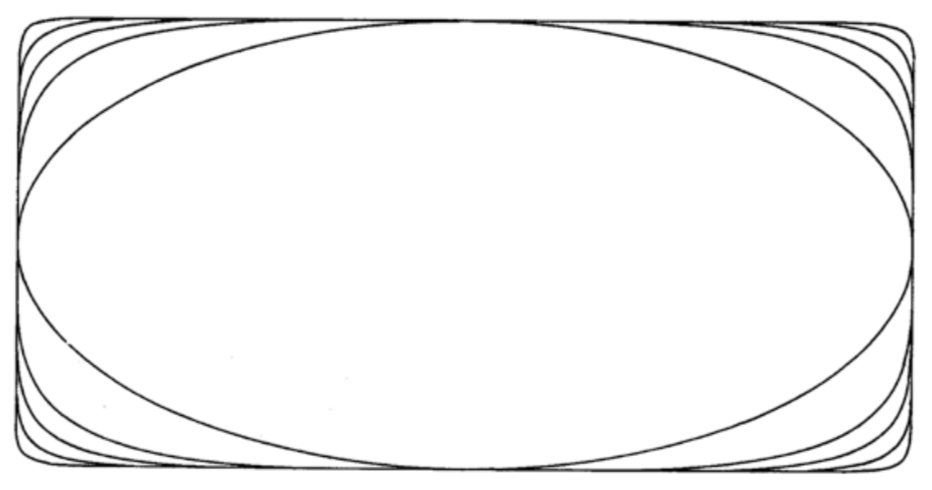
\includegraphics[width=0.5\textwidth]{Images/Elliptic_shapes.png}
%    \caption{Super-elliptic cross sections for aspect ratio c = 0.5. Curves from inside: n = 1, 2, 3, 5, 10}
%    \label{fig:elliptic_shapes}
%\end{figure}

%\nomenclature[G]{$\sigma_m$}{Normalized minimum wall shear stress \nomunit{[$-$]}}
%\nomenclature[A]{$c$}{Aspect ratio \nomunit{[$-$]}}

%\noindent The interest of corner rounding is shown by the minimum shear stress ($\sigma_m$) near a rounded corner. As said, with n=$\infty$ the curve approaches the values of a rectangular duct where $\sigma_n$=0 near the corners. The values of $\sigma_n$ with different values of n and c are shown in figure \ref{fig:shapes_table}. Here \cite{Wang} compared different n values with four cases from left to right (c=1, c=0.75, c=0.5, c=0.25).


%\begin{figure}[ht!]
%    \centering
%    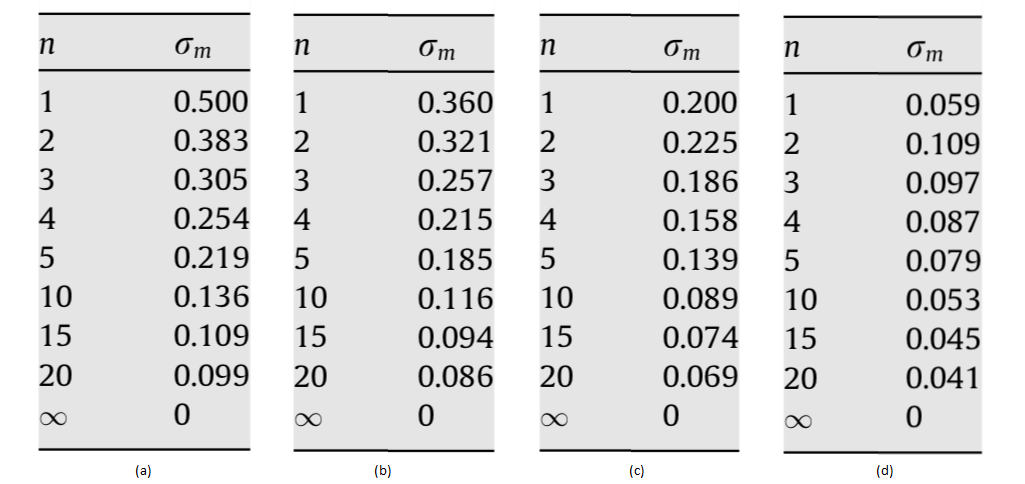
\includegraphics[width=0.8\textwidth]{Images/n_sigma_m.png}
%    \caption{Properties of a duct with aspect ratio (a) c=1, (b) c=0.75, (c) c=0.5, (d) c=0.25}
%    \label{fig:shapes_table}
%\end{figure}


%\noindent It is concluded that a rectangular shape with a high aspect ratio (low value of c) shows a decrease in shear stress near the rounded corners ($\sigma_m$) which connects to the founding of \cite{Decrop}. \newline

%\noindent \textit{Tests in an experimental setup are not done in the PhD thesis of \cite{Decrop} or in the investigation of \cite{Wang}, and so is an interesting part to investigate further. 




%Therefore it is chosen to go further with the tests of different overflow shapes, which can be translated to a mold design instead of a more complex setup for an experiment based on the decrease of air.}